\documentclass[12pt,a4paper]{article}%
\usepackage[T1]{fontenc}%
\usepackage[utf8]{inputenc}%
\usepackage{lmodern}%
\usepackage{textcomp}%
\usepackage{lastpage}%
\usepackage{geometry}%
\geometry{top=2.5cm,bottom=2.5cm,left=1.5cm,right=1.5cm}%
\usepackage{multicol}%
\usepackage{ragged2e}%
\usepackage{graphicx}%
\usepackage{amsmath}%
\usepackage{xcolor}%
\usepackage{caption}%
\usepackage{subcaption}%
\usepackage{enumitem}%
\usepackage{amssymb}%
\usepackage{multirow}%
\usepackage{tcolorbox}%
\usepackage{xparse}%
\usepackage{tikz}%
\usepackage{array}%
\usepackage{wasysym}%
\usepackage{float}%
\usepackage{lipsum}%
\usepackage{babel}%
\usepackage{wrapfig}%
\usepackage{tabularx}%
\usepackage{physics}%
\usepackage{mathdots}%
\usepackage{yhmath}%
\usepackage{cancel}%
\usepackage{color}%
\usepackage{gensymb}%
\usepackage{extarrows}%
\usepackage{booktabs}%
\usepackage{longtable}%
\usepackage{fancyhdr}%
%
%
%
\fancypagestyle{header}{%
\renewcommand{\headrulewidth}{0pt}%
\renewcommand{\footrulewidth}{0pt}%
% \fancyhead{%
% \centering{%
% \textbf{\huge Learn Basics Workbook - Math}
% }%
% }%
\fancyfoot{%
\noindent\rule{\textwidth}{1pt}%
}%
\fancyfoot[L]{%
\vspace{0.5cm}%
\large www.learnbasics.fun%
\hspace{2.5cm}%
\large Workbook of Abhiskek .A%
% Class 8 A,Lotus Public School%
}%
\fancyfoot[R]{%
\vspace{0.5cm}%
\large Page {\thepage}}%
}%

\begin{document}%
\normalsize%
\newcommand{\img}[3]{\begin{figure}[h] \centering \includegraphics[ width = #1, height = #2]{#3} \end{figure}}%
\newcommand{\question}[1]{\vspace{2.5mm} \begin{raggedright} #1  \leavevmode \newline \end{raggedright}}%
\newcommand{\hints}[1]{\vspace{2.5mm} \begin{raggedright} \textbf{\underline{{Answer:}}}  \\ #1  \leavevmode \newline \end{raggedright} \rule{\textwidth}{0.15pt} }%
\newcommand{\questionID}[1]{\vspace{2.5mm} \begin{raggedright} \textbf{\underline{{Question: #1}}}   \\ \end{raggedright}}%
\newcommand{\qrdes}[1]{\hspace{5cm} \begin{minipage}{12cm} \vspace{0.25mm} \begin{raggedright} \textbf{#1}\\ \end{raggedright}\end{minipage}}%
\newcommand{\qr}[1]{\begin{minipage}{3cm} \includegraphics[width=2cm]{#1} \end{minipage} \rule{\textwidth}{0.15pt}}%
\newcommand{\mcqfourfour}[9]{\vspace{2.5mm} \begin{raggedright} \textbf{#1} #2 \hfill \textit{#7} \textit{#8}\\ #9 \begin{multicols}{4}{} (a) #3\\ \columnbreak (b) #4\\ \columnbreak (c) #5\\ \columnbreak (d) #6\\ \end{multicols} \end{raggedright}}%
\newcommand{\mcqfourtwo}[9]{\vspace{2.5mm} \begin{raggedright} \textbf{#1} #2 \hfill \textit{#7} \textit{#8}\\ #9 \begin{multicols}{2}{} (a) #3\\ (c) #5\\ \columnbreak (b) #4\\ (d) #6\\ \end{multicols} \end{raggedright}}%
\centering%
\normalsize%
\pagestyle{header}%
\begin{minipage}{\textwidth}%
\textbf{\huge Learn Basics Workbook - Math}
\linebreak%
\noindent\rule{\textwidth}{1pt}%
\vspace{0.2cm}\\
\centering%
\underline{%
\begin{large}%
\textbf{LaPIS Diagnostic Test Report {-} Math}%
\end{large}%
}%
\vspace{0.3cm}\\
{\renewcommand{\arraystretch}{4}%
\begin{tabular}{ | p{2cm} p{1cm} p{10cm}| }
\hline

\textbf{\LARGE Name } & \textbf{\large :} & \textbf{\large Abhishek .A}\\%
\textbf{\LARGE Class } & \textbf{\large :} & \textbf{\large 8}\\%
\textbf{\LARGE Section } & \textbf{\large :} & \textbf{\large A}\\%
\textbf{\LARGE School} & \textbf{\large :} & \textbf{\large Lotus Public School}\\%
\hline
\end{tabular}}
\vspace{1cm}\\
\noindent\rule{\textwidth}{1pt}%

\linebreak%
\vspace{0.5cm}\\
\underline{%
\begin{Large}%
\textbf{Abishek .A's Performance Report}%
\end{Large}%
}%
\linebreak%
\linebreak%
\includegraphics[ width = 10cm, keepaspectratio]{png_files/Abishek .A_science_Class8_bargraph.png}%
\linebreak%
\linebreak%
\end{minipage}%
\linebreak%
\newpage%
\centering%
\begin{Large}%
\textbf{Abishek .A's Study Planner}%
\end{Large}%
\linebreak%
\noindent\rule{\textwidth}{2pt}%
\vspace{0.5cm} \\
\begin{longtable}{| l | l| l | l | l | l |}%
\hline%
Date&Topic Planned&Q Number&Teacher Remark&Teacher Sign&Parent Sign\\[1.5ex]%
\hline%
\endhead%
\hline%
 & & & & & \\[1.5ex]%
\hline%
 & & & & & \\[1.5ex]%
\hline%
 & & & & & \\[1.5ex]%
\hline%
 & & & & & \\[1.5ex]%
\hline%
 & & & & & \\[1.5ex]%
\hline%
 & & & & & \\[1.5ex]%
\hline%
 & & & & & \\[1.5ex]%
\hline%
 & & & & & \\[1.5ex]%
\hline%
 & & & & & \\[1.5ex]%
\hline%
 & & & & & \\[1.5ex]%
\hline%
 & & & & & \\[1.5ex]%
\hline%
 & & & & & \\[1.5ex]%
\hline%
 & & & & & \\[1.5ex]%
\hline%
 & & & & & \\[1.5ex]%
\hline%
 & & & & & \\[1.5ex]%
\hline%
 & & & & & \\[1.5ex]%
\hline%
 & & & & & \\[1.5ex]%
\hline%
 & & & & & \\[1.5ex]%
\hline%
 & & & & & \\[1.5ex]%
\hline%
 & & & & & \\[1.5ex]%
\hline%
 & & & & & \\[1.5ex]%
\hline%
\end{longtable}%
Teacher's Feedback to Student%
\linebreak%
\linebreak%
% \framebox[15cm][25]{\vspace{10cm}}%
\framebox(15cm,1.8cm){}
\linebreak%
\linebreak%
\linebreak%
\linebreak%
\begin{minipage}[l]{0.45\textwidth}%
\flushleft%
\centering%
\par\noindent\rule{40mm}{0.4pt} \linebreak Class Teacher Signature%
\end{minipage}%
\begin{minipage}[l]{0.45\textwidth}%
\flushleft%
\centering%
\par\noindent\rule{40mm}{0.4pt} \linebreak Principal Signature%
\end{minipage}%
\newpage%

\newpage%
\noindent\rule{\textwidth}{2pt}%
\linebreak%
\centering%
\begin{Large}%
\textbf{Algebra}%
\end{Large}%
\linebreak%
\noindent\rule{\textwidth}{2pt}%
\begin{center}%
\medskip%
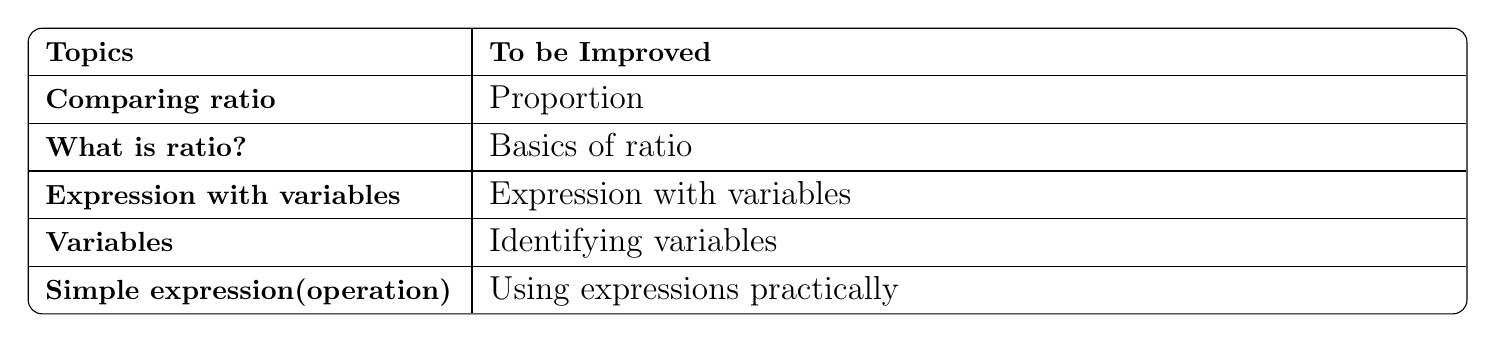
\begin{tikzpicture}%
\node (table) [inner sep=0pt] {%
{\renewcommand{\arraystretch}{1.4}%
\begin{tabular}{  m{5.2cm} | m{12.2cm}  } %
\textbf{Topics} & \textbf{To be Improved}
        \\
        \hline%
\normalsize{ \textbf{Comparing ratio}} & \large{Proportion}%
\\
            \hline%
\normalsize{ \textbf{What is ratio?}} & \large{Basics of ratio}%
\\
            \hline%
\normalsize{ \textbf{Expression with variables}} & \large{Expression with variables}%
\\
            \hline%
\normalsize{ \textbf{Variables}} & \large{Identifying variables}%
\\
            \hline%
\normalsize{\textbf{Simple expression(operation)}} & \large{Using expressions practically}%
\end{tabular}}};%
\draw [rounded corners=.5em] (table.north west) rectangle (table.south east);%
\end{tikzpicture}%
\end{center}%
\questionID {C6MDT22A}%
\question
{
Find the missing number?\\
\tikzset{every picture/.style={line width=0.75pt}} 

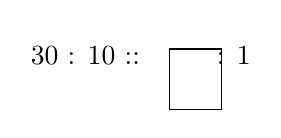
\begin{tikzpicture}[x=0.75pt,y=0.75pt,yscale=-1,xscale=1]


\draw   (91,60) -- (116,60) -- (116,89) -- (91,89) -- cycle ;

\draw (23,50) node [anchor=north west][inner sep=0.75pt]   [align=left] {\\30 : 10 ::  \ \ \ \ \ \ \ : 1 };


\end{tikzpicture}}%
\hints{ 

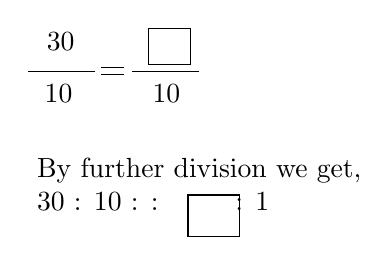
\begin{tikzpicture}[x=0.75pt,y=0.75pt,yscale=-1,xscale=1]



\draw   (105,132) -- (130,132) -- (130,152.02) -- (105,152.02) -- cycle ;
 
\draw    (28,72.67) -- (60.29,72.67) ;

\draw   (86,51.67) -- (106.29,51.67) -- (106.29,69.15) -- (86,69.15) -- cycle ;
 
\draw    (78,72.67) -- (110.29,72.67) ;
 
\draw    (63,70.67) -- (74.29,70.67) ;
 
\draw    (63,74.15) -- (74.29,74.15) ;



\draw (31,113) node [anchor=north west][inner sep=0.75pt]   [align=left] {By further division we get,
\\30 : 10 : : \ \ \ \ \ \ \ : 1 };

\draw (35.67,52.67) node [anchor=north west][inner sep=0.75pt]   [align=left] {30};

\draw (34.67,77.67) node [anchor=north west][inner sep=0.75pt]   [align=left] {10};

\draw (86.67,77.67) node [anchor=north west][inner sep=0.75pt]   [align=left] {10};


\end{tikzpicture}}%
\questionID {C6MDT22B}%
\question
{Find the value of y.\\
12 mangoes : 3 mangoes : : Rs.60 : Rs.y}%
\hints{\tikzset{every picture/.style={line width=0.75pt}} 

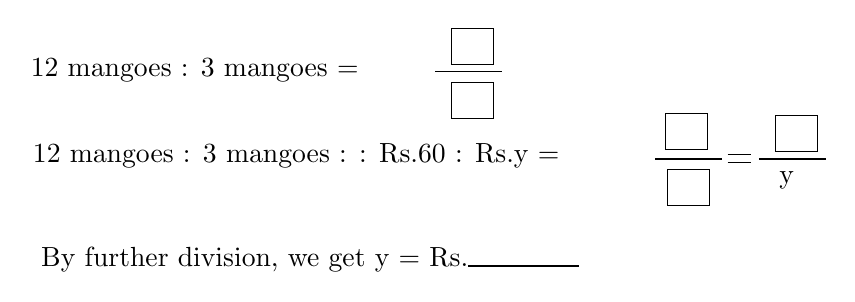
\begin{tikzpicture}[x=0.75pt,y=0.75pt,yscale=-1,xscale=1]

\draw    (316,77.67) -- (348.29,77.67) ;

\draw   (374,56.67) -- (394.29,56.67) -- (394.29,74.15) -- (374,74.15) -- cycle ;
\draw    (366,77.67) -- (398.29,77.67) ;

\draw    (351,75.67) -- (362.29,75.67) ;
 
\draw    (351,79.15) -- (362.29,79.15) ;

 
\draw   (218,14.67) -- (238.29,14.67) -- (238.29,32.15) -- (218,32.15) -- cycle ;
 
\draw    (210,35.67) -- (242.29,35.67) ;
 
\draw   (218,40.67) -- (238.29,40.67) -- (238.29,58.15) -- (218,58.15) -- cycle ;
 
\draw   (321,55.67) -- (341.29,55.67) -- (341.29,73.15) -- (321,73.15) -- cycle ;
 
\draw   (322,82.67) -- (342.29,82.67) -- (342.29,100.15) -- (322,100.15) -- cycle ;


\draw (14,28) node [anchor=north west][inner sep=0.75pt]   [align=left] {12 mangoes : 3 mangoes = };

\draw (15,69) node [anchor=north west][inner sep=0.75pt]   [align=left] {12 mangoes : 3 mangoes : : Rs.60 : Rs.y = \ \ };

\draw (374.67,82.67) node [anchor=north west][inner sep=0.75pt]   [align=left] { y};

\draw (19,119) node [anchor=north west][inner sep=0.75pt]   [align=left] {By further division, we get y = Rs.\rule{40pt}{0.5pt}};


\end{tikzpicture}}%
\questionID {C6MDT22C}%
\question
{Karun earns Rs.35000 per month. Determine if the ratio of Karun’s monthly salary : Karun’s two month salary : : Karun’s half year income : Karun’s annual income is proportional.}%
\hints{Karun’s salary per month = Rs. \rule{40pt}{0.5pt}\\
Karun’s two month salary = Rs.\rule{40pt}{0.5pt}\\
Half year = \rule{40pt}{0.5pt}months\\
Karun’s half year income = Rs.\rule{40pt}{0.5pt} x \rule{40pt}{0.5pt} = \rule{40pt}{0.5pt}\\
1 year = \rule{40pt}{0.5pt} months\\
Karun’s annual income = Rs.\rule{40pt}{0.5pt}x \rule{40pt}{0.5pt} = \rule{40pt}{0.5pt}
\\
Checking whether the ratio of Karun’s monthly salary : Karun’s two month salary : : Karun’s half year income : Karun’s annual income is proportional. 
}%
\questionID {C6MDT18A}%
\question
{Which of the below given boxes are equal to the ratio 3 : 5\\ \bigskip{}


\tikzset{every picture/.style={line width=0.75pt}}        

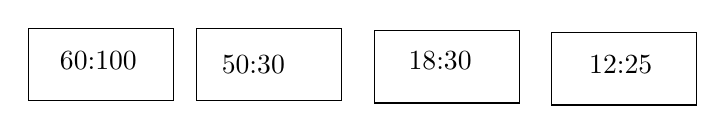
\begin{tikzpicture}[x=0.75pt,y=0.75pt,yscale=-1,xscale=1]
\draw   (92,101) -- (161.8,101) -- (161.8,136) -- (92,136) -- cycle ;
\draw   (173,101) -- (242.8,101) -- (242.8,136) -- (173,136) -- cycle ;
\draw   (259,102) -- (328.8,102) -- (328.8,137) -- (259,137) -- cycle ;
\draw   (344,103) -- (413.8,103) -- (413.8,138) -- (344,138) -- cycle ;
\draw (106,111) node [anchor=north west][inner sep=0.75pt]   [align=left] {60:100};
\draw (184,113) node [anchor=north west][inner sep=0.75pt]   [align=left] {50:30};
\draw (274,111) node [anchor=north west][inner sep=0.75pt]   [align=left] {18:30};
\draw (361,113) node [anchor=north west][inner sep=0.75pt]   [align=left] {12:25};
\end{tikzpicture}

}%
\hints{Comparing the two quantities in terms of ‘how many times’. This comparison is known as the \rule{80pt}{0.5pt}\\
\bigskip


\tikzset{every picture/.style={line width=0.75pt}}
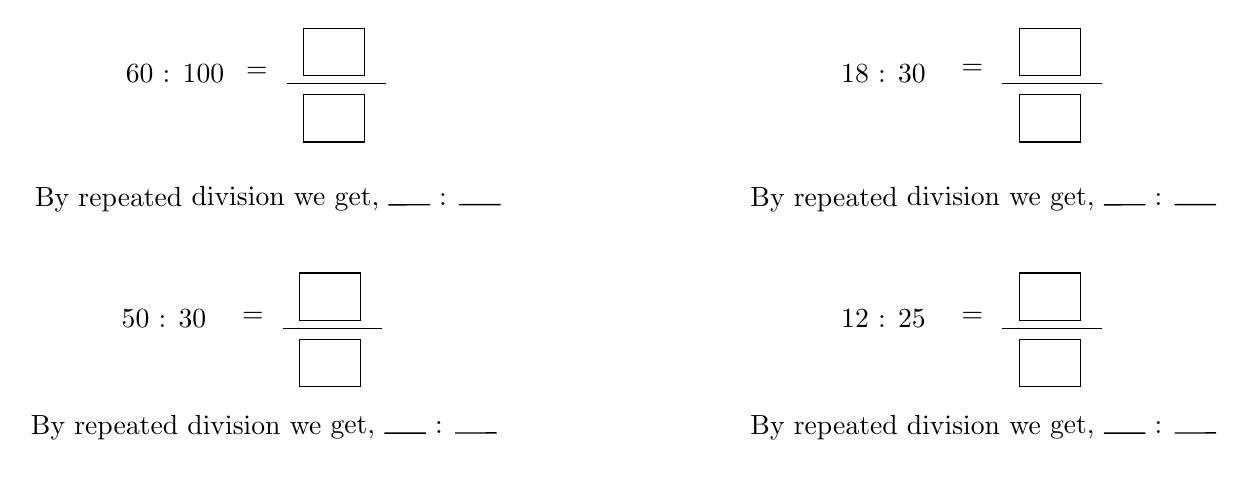
\begin{tikzpicture}[x=0.75pt,y=0.75pt,yscale=-1,xscale=1]


\draw   (163.01,127.63) -- (192.41,127.63) -- (192.41,104.74) -- (163.01,104.74) -- cycle ;

\draw    (154.8,131.53) -- (202.8,131.53) ;

\draw   (163.01,159.57) -- (192.41,159.57) -- (192.41,136.67) -- (163.01,136.67) -- cycle ;



\draw   (161.01,245.56) -- (190.41,245.56) -- (190.41,222.67) -- (161.01,222.67) -- cycle ;
\draw    (152.8,249.46) -- (200.8,249.46) ;
\draw   (161.01,277.5) -- (190.41,277.5) -- (190.41,254.6) -- (161.01,254.6) -- cycle ;
\draw   (507.68,127.63) -- (537.08,127.63) -- (537.08,104.74) -- (507.68,104.74) -- cycle ;
\draw    (499.47,131.53) -- (547.47,131.53) ;
\draw   (507.68,159.57) -- (537.08,159.57) -- (537.08,136.67) -- (507.68,136.67) -- cycle ;
\draw   (507.68,245.56) -- (537.08,245.56) -- (537.08,222.67) -- (507.68,222.67) -- cycle ;
\draw    (499.47,249.46) -- (547.47,249.46) ;
\draw   (507.68,277.5) -- (537.08,277.5) -- (537.08,254.6) -- (507.68,254.6) -- cycle ;
\draw (134,122.32) node [anchor=north west][inner sep=0.75pt]   [align=left] {=};
\draw (32.24,180) node [anchor=north west][inner sep=0.75pt]  [rotate=-359.88] [align=left] {By repeated division we get, \rule{15pt}{0.5pt} : \rule{15pt}{0.5pt}\\};
\draw (76,121) node [anchor=north west][inner sep=0.75pt]   [align=left] {60 : 100};
\draw (74,238.93) node [anchor=north west][inner sep=0.75pt]   [align=left] {50 : 30};
\draw (30.24,290) node [anchor=north west][inner sep=0.75pt]  [rotate=-359.88] [align=left] {By repeated division we get, \rule{15pt}{0.5pt} : \rule{15pt}{0.5pt}\\};
\draw (132,240.25) node [anchor=north west][inner sep=0.75pt]   [align=left] {=};
\draw (420.67,238.93) node [anchor=north west][inner sep=0.75pt]   [align=left] {12 : 25};
\draw (376.9,180) node [anchor=north west][inner sep=0.75pt]  [rotate=-359.88] [align=left] {By repeated division we get, \rule{15pt}{0.5pt} : \rule{15pt}{0.5pt}\\};
\draw (478.67,121) node [anchor=north west][inner sep=0.75pt]   [align=left] {=};
\draw (420.67,121) node [anchor=north west][inner sep=0.75pt]   [align=left] {18 : 30};
\draw (376.9,290) node [anchor=north west][inner sep=0.75pt]  [rotate=-359.88] [align=left] {By repeated division we get, \rule{15pt}{0.5pt} : \rule{15pt}{0.5pt}\\};
\draw (478.67,240.25) node [anchor=north west][inner sep=0.75pt]   [align=left] {=};
\end{tikzpicture}
 }%
\questionID {C6MDT18B}%
\question
{Find the ratio of 150cm to 1.2m in simplest form.}%
\hints{
\begin{align*}
    \text{1 meter} &= \rule{40pt}{0.5pt}\\
    \text{1.2 meter} &= \text{\rule{40pt}{0.5pt} x \rule{40pt}{0.5pt} cm} \\
    \text{1.2 meter} &= \text{\rule{40pt}{0.5pt}cm}\\
    \text{150cm : 1.2m} &= 150 :\rule{40pt}{0.5pt}\\
\end{align*}
By repeated division we get, \rule{40pt}{0.5pt} : \rule{40pt}{0.5pt} }%
\questionID {C6MDT18C}%
\question
{The height and base of a triangular sign board is 32cm and 40cm respectively. What is the ratio of height to the base ?}%
\hints{
\begin{align*}
{\text{Height of a triangular sign board}} &= \rule{40pt}{0.5pt} \\
\text{Base of a triangular sign board} &= \rule{40pt}{0.5pt}\\
\text{Ratio of height to base} &= \rule{40pt}{0.5pt}:\rule{40pt}{0.5pt}\\
\text {By repeating division, we get } &  \rule{40pt}{0.5pt}:\rule{40pt}{0.5pt}\\
\end{align*} 

}%
\questionID {C6MDT19A}%
\question
{Determine if the following are in proportion.40, 240, 100, 600}%
\hints{\bigskip
{
\tikzset{every picture/.style={line width=1pt}}       
\begin{tikzpicture}[x=1pt,y=1pt,yscale=-1,xscale=1]
\newline
\draw   (96,70) -- (124,70) -- (124,98) -- (96,98) -- cycle ;
\draw    (86,108) -- (140,108) ;
\draw   (96,117) -- (124,117) -- (124,145) -- (96,145) -- cycle ;

\draw   (184,70) -- (212,70) -- (212,98) -- (184,98) -- cycle ;
\draw    (174,108) -- (228,108) ;
\draw   (184,117) -- (212,117) -- (212,145) -- (184,145) -- cycle ;


\draw   (97,197) -- (125,197) -- (125,225) -- (97,225) -- cycle ;
\draw    (87,235) -- (141,235) ;
\draw   (97,244) -- (125,244) -- (125,272) -- (97,272) -- cycle ;

\draw   (185,197) -- (213,197) -- (213,225) -- (185,225) -- cycle ;
\draw    (175,235) -- (229,235) ;
\draw   (185,244) -- (213,244) -- (213,272) -- (185,272) -- cycle ;




\draw (148,101) node [anchor=north west][inner sep=0.75pt]   [align=left] {=};
\draw (149,228) node [anchor=north west][inner sep=0.75pt]   [align=left] {=};
\draw (89,36) node [anchor=north west][inner sep=0.75pt]   [align=left] {40 : 240 : : 100 : 60};
\draw (89,165) node [anchor=north west][inner sep=0.75pt]   [align=left] {By repeated division, we get};
\draw (91,291) node [anchor=north west][inner sep=0.75pt]   [align=left] {These numbers are proportional / not proportional};
\end{tikzpicture}
}}%
\questionID {C6MDT19B}%
\question
{The ratio of student who chose Sanskrit as their second language to French as their second language is 13 : 17 where, 85 students chose French as their second language. How many students chose Sanskrit as their second language?}%
\hints{The ratio of student choose Sanskrit : The ratio of student choose French  = \rule{20pt}{0.5pt} : \rule{20pt}{0.5pt}\\
Number of students who choose French as their second language is \rule{40pt}{0.5pt}\\
\begin{center}

\tikzset{every picture/.style={line width=0.75pt}}

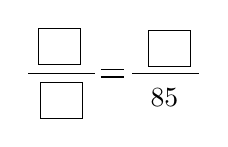
\begin{tikzpicture}[x=0.75pt,y=0.75pt,yscale=-1,xscale=1]

\draw    (430,83.67) -- (462.29,83.67) ;

\draw   (488,62.67) -- (508.29,62.67) -- (508.29,80.15) -- (488,80.15) -- cycle ;

\draw    (480,83.67) -- (512.29,83.67) ;

\draw    (465,81.67) -- (476.29,81.67) ;

\draw    (465,85.15) -- (476.29,85.15) ;

\draw   (436,87.67) -- (456.29,87.67) -- (456.29,105.15) -- (436,105.15) -- cycle ;

\draw   (435,61.67) -- (455.29,61.67) -- (455.29,79.15) -- (435,79.15) -- cycle ;

\draw (487.67,89.67) node [anchor=north west][inner sep=0.75pt]   [align=left] {85};


\end{tikzpicture}
\end{center}
Number of students who choose Sanskrit as their second language is \rule{40pt}{0.5pt}

}%
\questionID {C6MDT19C}%
\question
{Determine if the following ratios form a proportion.\\  120grams to 1.2kg and 6 sec to 1 minute.}%
\hints{
\begin{align*}
   \text{1 kg} &= \text{\rule{40pt}{0.5pt} grams}\\ 
   \text{1.2 kg} &= \text{1.2 x \rule{40pt}{0.5pt}}\\ 
   \text{1.2 kg} &= \text{\rule{40pt}{0.5pt} grams}\\ 
   \text{120 gram : 1.2kg} &= \text{\rule{80pt}{0.5pt} : \rule{80pt}{0.5pt}}\\ 
  \text{1 minute} &= \text{\rule{40pt}{0.5pt} seconds}\\  
  \text{6 sec : 1 minute} &= \text{\rule{80pt}{0.5pt} : \rule{80pt}{0.5pt}}\\  
\end{align*}
These ratios are proportional/ not proportional
}%
\questionID {C6MDT15A}%
\question
{The weight of each apple is given below. Find the total weight of all the apples. \img{12cm}{5cm}{Q15A.png}  }%
\hints{Total given number of apples are \rule{80pt}{0.5pt}. \\
 The weight of each apple are \rule{80pt}{0.5pt}, \rule{80pt}{0.5pt}, \rule{80pt}{0.5pt}. \\
Total weight of the given apples = Apple 1 ( \rule{80pt}{0.5pt} ) Apple 2 ( \rule{80pt}{0.5pt} ) Apple 3. 
}%
\questionID {C6MDT15B}%
\question
{Express the statement. \\ 
\begin{enumerate}[label=(\roman*)]
\item - 4 is multiplied by m from which 3 is subtracted. 
\item 6 is added to y, this sum is divided by 8.
\end{enumerate}}%
\hints{

\tikzset{every picture/.style={line width=0.75pt}}        

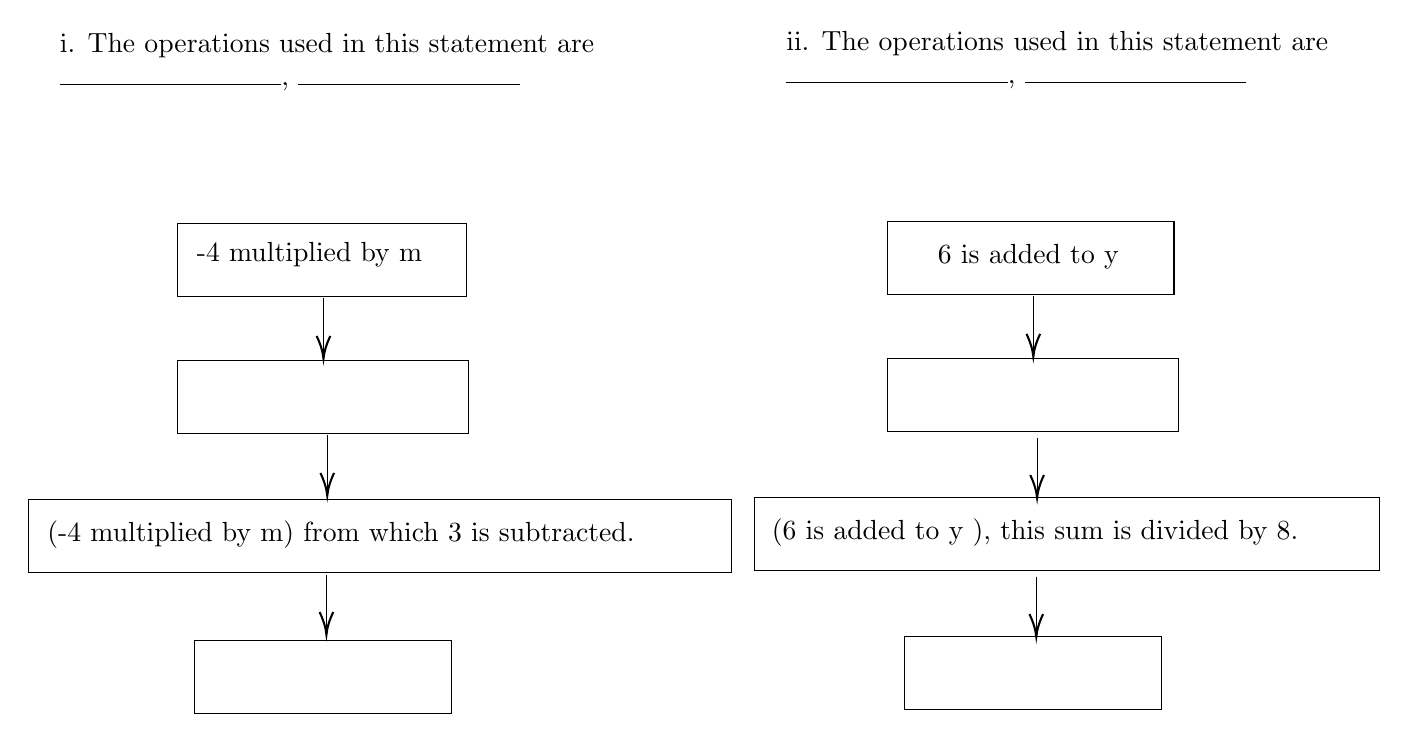
\begin{tikzpicture}[x=0.75pt,y=0.75pt,yscale=-1,xscale=1]


\draw   (420,108) -- (558,108) -- (558,143.21) -- (420,143.21) -- cycle ;

\draw    (490.25,144.21) -- (490.25,157.21) -- (490.25,171.21) ;
\draw [shift={(490.25,173.21)}, rotate = 270] [color={rgb, 255:red, 0; green, 0; blue, 0 }  ][line width=0.75]    (10.93,-3.29) .. controls (6.95,-1.4) and (3.31,-0.3) .. (0,0) .. controls (3.31,0.3) and (6.95,1.4) .. (10.93,3.29)   ;

\draw   (420,174) -- (560,174) -- (560,209.21) -- (420,209.21) -- cycle ;

\draw   (356,241) -- (657,241) -- (657,276.21) -- (356,276.21) -- cycle ;

\draw   (428,308) -- (552,308) -- (552,343.21) -- (428,343.21) -- cycle ;

\draw    (492.07,212.21) -- (492.07,225.21) -- (492.07,239.21) ;
\draw [shift={(492.07,241.21)}, rotate = 270] [color={rgb, 255:red, 0; green, 0; blue, 0 }  ][line width=0.75]    (10.93,-3.29) .. controls (6.95,-1.4) and (3.31,-0.3) .. (0,0) .. controls (3.31,0.3) and (6.95,1.4) .. (10.93,3.29)   ;

\draw    (491.67,279.21) -- (491.67,292.21) -- (491.67,306.21) ;
\draw [shift={(491.67,308.21)}, rotate = 270] [color={rgb, 255:red, 0; green, 0; blue, 0 }  ][line width=0.75]    (10.93,-3.29) .. controls (6.95,-1.4) and (3.31,-0.3) .. (0,0) .. controls (3.31,0.3) and (6.95,1.4) .. (10.93,3.29)   ;

\draw   (78,109) -- (217,109) -- (217,144.21) -- (78,144.21) -- cycle ;

\draw    (148.25,145.21) -- (148.25,158.21) -- (148.25,172.21) ;
\draw [shift={(148.25,174.21)}, rotate = 270] [color={rgb, 255:red, 0; green, 0; blue, 0 }  ][line width=0.75]    (10.93,-3.29) .. controls (6.95,-1.4) and (3.31,-0.3) .. (0,0) .. controls (3.31,0.3) and (6.95,1.4) .. (10.93,3.29)   ;

\draw   (78,175) -- (218,175) -- (218,210.21) -- (78,210.21) -- cycle ;
 
\draw    (150.07,211.21) -- (150.07,224.21) -- (150.07,238.21) ;
\draw [shift={(150.07,240.21)}, rotate = 270] [color={rgb, 255:red, 0; green, 0; blue, 0 }  ][line width=0.75]    (10.93,-3.29) .. controls (6.95,-1.4) and (3.31,-0.3) .. (0,0) .. controls (3.31,0.3) and (6.95,1.4) .. (10.93,3.29)   ;

\draw   (6,242) -- (345,242) -- (345,277.21) -- (6,277.21) -- cycle ;

\draw    (149.67,278.21) -- (149.67,291.21) -- (149.67,305.21) ;
\draw [shift={(149.67,307.21)}, rotate = 270] [color={rgb, 255:red, 0; green, 0; blue, 0 }  ][line width=0.75]    (10.93,-3.29) .. controls (6.95,-1.4) and (3.31,-0.3) .. (0,0) .. controls (3.31,0.3) and (6.95,1.4) .. (10.93,3.29)   ;

\draw   (86,310) -- (210,310) -- (210,345.21) -- (86,345.21) -- cycle ;


\draw (20,16) node [anchor=north west][inner sep=0.75pt]   [align=left] {i. The operations used in this statement are \\\rule{80pt}{0.5pt}, \rule{80pt}{0.5pt}};

\draw (370,15) node [anchor=north west][inner sep=0.75pt]   [align=left] {ii. The operations used in this statement are\\\rule{80pt}{0.5pt}, \rule{80pt}{0.5pt}};

\draw (14,251) node [anchor=north west][inner sep=0.75pt]   [align=left] {(-4 multiplied by m) from which 3 is subtracted. };

\draw (443,118) node [anchor=north west][inner sep=0.75pt]   [align=left] {6 is added to y};

\draw (86,117) node [anchor=north west][inner sep=0.75pt]   [align=left] {\mbox{-}4 multiplied by m };

\draw (363,250) node [anchor=north west][inner sep=0.75pt]   [align=left] {(6 is added to y ), this sum is divided by 8. };


\end{tikzpicture}

}%
\questionID {C6MDT15C}%
\question
{Arun is ‘x’ years old. Karan is 2 years less than twice the age of Arun. Express Karan’s age.}%
\hints{Age of Arun is \rule{80pt}{0.5pt}.\\
Twice the age of Arun can be written as \rule{80pt}{0.5pt}. \\
Karan’s age = 2 less than twice the age of Arun = \rule{80pt}{0.5pt} .
}%
\questionID {C6MDT14A}%
\question
{Pick the correct answer.\\\rule{80pt}{0.5pt} is an alphabet that represents an unknown number or quantity. (Variable/Expression).}%
\hints{Unknown values are represented by an alphabet or a symbol is called as \rule{80pt}{0.5pt} and it’s value is not \rule{80pt}{0.5pt}. 
}%
\questionID {C6MDT14B}%
\question
{Tick the boxes which have expressions with a variables
\begin{center}




\tikzset{every picture/.style={line width=0.75pt}}        

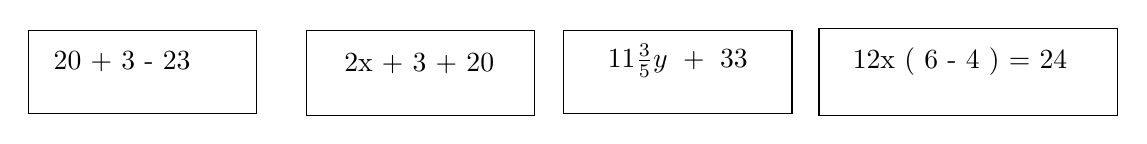
\begin{tikzpicture}[x=0.75pt,y=0.75pt,yscale=-1,xscale=1]


 
\draw   (44,95) -- (154,95) -- (154,135) -- (44,135) -- cycle ;

\draw   (178,95) -- (288,95) -- (288,136) -- (178,136) -- cycle ;

\draw   (302,95) -- (412,95) -- (412,135) -- (302,135) -- cycle ;

\draw   (425,94) -- (569,94) -- (569,136) -- (425,136) -- cycle ;



\draw (55,104) node [anchor=north west][inner sep=0.75pt]   [align=left] {20 + 3 - 23};

\draw (195,105) node [anchor=north west][inner sep=0.75pt]   [align=left] {2x + 3 + 20};

\draw (336,98) node [anchor=north west][inner sep=0.75pt]   [align=left] {};

\draw (440,102) node [anchor=north west][inner sep=0.75pt]   [align=left] {12x ( 6 - 4 ) = 24};

\draw (322,100.4) node [anchor=north west][inner sep=0.75pt]  [font=\normalsize]  {$11\frac{3}{5} y\ +\ 33$};


\end{tikzpicture}
\end{center}}%
\hints{The variables are denoted by \rule{80pt}{0.5pt} (alphabets/ symbol / number).\\
The expressions in the given boxes are \rule{160pt}{0.5pt}.\\
The expression which contains variable are \rule{160pt}{0.5pt}.
}%
\questionID {C6MDT14C}%
\question
{There are x number of students in a classroom where 14 students went for swimming class, 9 students went for music class, 3 students were in library. Write an expression for the remaining number of students in the classroom.}%
\hints{Total number of students in a class room are \rule{80pt}{0.5pt}.\\
 The students who went for swimming class are \rule{80pt}{0.5pt} \\
 Students went for music class are \rule{80pt}{0.5pt} \\
 The students went to library are \rule{80pt}{0.5pt} \\
Number of remaining students = Total number of students in a class room (-) Total number of 									     students outside the class
}%
\questionID {C6MDT17A}%
\question
{\img{18cm}{3cm}{Q17A.png}}%
\hints{The total distance is \rule{80pt}{0.5pt}.\\
A man covered \rule{80pt}{0.5pt} kilometers from the starting point initially.\\
\begin{align*}
  \text{Remaining distance to reach ending point} &= \text{Total distance \rule{20pt}{0.5pt} initial distance covered.}\\ 
  \text{Remaining distance} &= \text{\rule{80pt}{0.5pt}}.
\end{align*}


}%
\questionID {C6MDT17B}%
\question
{There are a total of 120 toffees in two jars. One jar is bigger than the other and it contain 86 toffees. How many toffees are there in the small jar.}%
\hints{The total number of toffees are \rule{80pt}{0.5pt}.\\
Bigger jar contains \rule{80pt}{0.5pt} toffees.\\
Number of toffees in small jar = Total number of toffees \rule{80pt}{0.5pt} (×/÷/-) Number of toffees in big jar.
}%
\questionID {C6MDT17C}%
\question
{A cobbler mends 12 shoes a day except sunday. On Sunday he mends only 4 shoes. What is the total number of shoes the cobbler mends in a week.}%
\hints{


Total number of days in a week \rule{80pt}{0.5pt}.\\
The cobbler mends \rule{80pt}{0.5pt} shoes per day(except Sunday).\\


\begin{align*}
   \text{ Total shoes mends on a week (except Sunday)}  &=\text{\rule{160pt}{0.5pt} × \rule{80pt}{0.5pt}}\\
    &= \text{\rule{160pt}{0.5pt}.}\\
\end{align*}

On Sunday he mends only \rule{80pt}{0.5pt}.\\

\begin{align*}
\text{Total number of shoes the cobbler mends in a week} & = \text{shoe mends in other days}\\
& = \text{\rule{80pt}{0.5pt} shoe mends on Sunday}\\
 \text{Total number of shoes the cobbler mends in a week} & = \text{\rule{80pt}{0.5pt}.}\\
\end{align*}

}%
\noindent\rule{\textwidth}{2pt}%
\linebreak%
\centering%
\begin{Large}%
\textbf{Basic Arithmetic}%
\end{Large}%
\linebreak%
\noindent\rule{\textwidth}{2pt}%
\begin{center}%
\medskip%
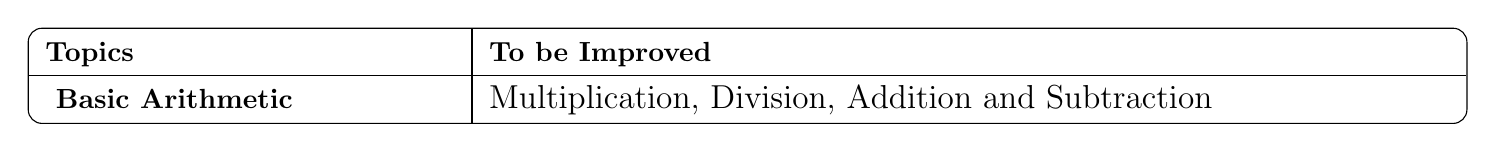
\begin{tikzpicture}%
\node (table) [inner sep=0pt] {%
{\renewcommand{\arraystretch}{1.4}%
\begin{tabular}{  m{5.2cm} | m{12.2cm}  } %
\textbf{Topics} & \textbf{To be Improved}
        \\
        \hline%
\normalsize{\textbf{ Basic Arithmetic}} & \large{Multiplication, Division, Addition and Subtraction}%
\end{tabular}}};%
\draw [rounded corners=.5em] (table.north west) rectangle (table.south east);%
\end{tikzpicture}%
\end{center}%
\questionID {C6MDT27A}%
\question
{Solve : 8 x 10 x 11}%
\hints{Changing the grouping in which we multiply numbers does not change the product.\\
(a x b) x c = \rule{80pt}{0.5pt}\\
 This property is called  \rule{80pt}{0.5pt}\\
8 x 10 = \rule{80pt}{0.5pt}\\
\rule{20pt}{0.5pt} x 11 =  \rule{80pt}{0.5pt}\\
8 x 10 x 11 = \rule{80pt}{0.5pt}
}%
\questionID {C6MDT27B}%
\question
{Solve : \\
1562 × 48}%
\hints{\begin{table}[H]
  \centering
\renewcommand{\arraystretch}{1.15}
    \begin{tabular}{p{0.3cm}p{0.5cm}p{0.5cm}p{0.5cm}p{0.2cm}}
            & 1 & 5 & 6 & 2\\
            $\times$ &  &  & 4 & 8  \\
        \hline
       & & & &  \\
              &  & & &    \\
                       \hline
      &   & & &\\ 
         \hline
         \end{tabular}
\end{table}
Therefore, 1562 × 48 = \rule{80pt}{0.5pt} }%
\questionID {C6MDT27C}%
\question
{Fill in the blanks with the correct answer.\\
156 × \rule{20pt}{0.5pt} = 1872\\

\begin{center}
    \tikzset{every picture/.style={line width=0.75pt}} 

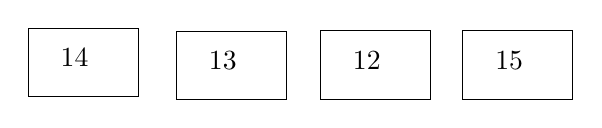
\begin{tikzpicture}[x=0.75pt,y=0.75pt,yscale=-1,xscale=1]


\draw   (143,206.02) -- (196,206.02) -- (196,239) -- (143,239) -- cycle ;


\draw   (214.4,207.43) -- (267.4,207.43) -- (267.4,240.42) -- (214.4,240.42) -- cycle ;


\draw   (283.8,207.23) -- (336.8,207.23) -- (336.8,240.22) -- (283.8,240.22) -- cycle ;


\draw   (352.4,207.23) -- (405.4,207.23) -- (405.4,240.22) -- (352.4,240.22) -- cycle ;




\draw (157.4,214.8) node [anchor=north west][inner sep=0.75pt]   [align=left] {14};

\draw (228.8,216.22) node [anchor=north west][inner sep=0.75pt]   [align=left] {13};

\draw (298.2,216.02) node [anchor=north west][inner sep=0.75pt]   [align=left] {12};

\draw (366.8,216.02) node [anchor=north west][inner sep=0.75pt]   [align=left] {15};


\end{tikzpicture}
\end{center}
}%
\hints{
\begin{table}[H]
  \centering
\renewcommand{\arraystretch}{1.15}
    \begin{tabular}{p{0.3cm}p{0.3cm}p{0.3cm}p{0.3cm}p{0.5cm}
    p{0.3cm}p{0.3cm}p{0.3cm}p{0.3cm}p{0.5cm}
    p{0.3cm}p{0.3cm}p{0.3cm}p{0.3cm}p{0.5cm}
    p{0.3cm}p{0.3cm}p{0.3cm}p{0.3cm}p{0.5cm}
    p{0.3cm}p{0.3cm}p{0.3cm}p{0.3cm}} 
   
            & 1 & 5 & 6 & && 1 & 5 & 6 & & & 1 & 5 & 6 & & &1 & 5 & 6 \\
            $\times$ &  & 1 & 4 & & 
            $\times$ &  & 1 & 3 & & 
            $\times$ &  & 1 & 2 & &
            $\times$ & & 1 & 5 & \\
        \cline{1-4}\cline{6-9} \cline{11-14} \cline{16-19}
       & & & &  \\
       & & & &    \\
       \cline{1-4}\cline{6-9} \cline{11-14}\cline{16-19}
       & & & &\\ 
        \cline{1-4}\cline{6-9} \cline{11-14} \cline{16-19}
         \end{tabular}
\end{table}

Therefore, 156 × \rule{20pt}{0.5pt} = 1872
}%
\questionID {C6MDT25A}%
\question
{Solve
$\frac{25 \times 12}{5}$}%
\hints{This can be also written as $\frac{25}{5}$ $\times$ 12\\
25 is divided by 5 and the answer is multiplied by \rule{40pt}{0.5pt}\\
The final answer is \rule{40pt}{0.5pt}
}%
\questionID {C6MDT25B}%
\question
{What is the remainder of 558 ÷ 5 ?}%
\hints{
\begin{center}
    
\tikzset{every picture/.style={line width=0.75pt}} 
\begin{tikzpicture}[x=0.75pt,y=0.75pt,yscale=-1,xscale=1]


\draw    (57,36.02) -- (57,166) ;

\draw    (57,36.02) -- (226,36.02) ;

\draw    (57,165) -- (226,165) ;
 
\draw    (57,123.02) -- (226,123.02) ;

\draw    (60,231) -- (229,231) ;

\draw    (61,260) -- (230,260) ;


\draw    (102,28) -- (117,28) -- (135,28) ;

\draw    (150,28) -- (165,28) -- (183,28) ;

\draw    (225,245) -- (256,245) ;
\draw [shift={(258,245)}, rotate = 180] [color={rgb, 255:red, 0; green, 0; blue, 0 }  ][line width=0.75]    (10.93,-3.29) .. controls (6.95,-1.4) and (3.31,-0.3) .. (0,0) .. controls (3.31,0.3) and (6.95,1.4) .. (10.93,3.29)   ;


\draw (77,12) node [anchor=north west][inner sep=0.75pt]  [font=\large] [align=left] {1};

\draw (77,45) node [anchor=north west][inner sep=0.75pt]  [font=\large] [align=left] {5};

\draw (136,45) node [anchor=north west][inner sep=0.75pt]  [font=\large] [align=left] {5};

\draw (186,45) node [anchor=north west][inner sep=0.75pt]  [font=\large] [align=left] {8};

\draw (20,44) node [anchor=north west][inner sep=0.75pt]  [font=\large] [align=left] {5};

\draw (269,238) node [anchor=north west][inner sep=0.75pt]   [align=left] {Remainder};


\end{tikzpicture}
\end{center}
}%
\questionID {C6MDT25C}%
\question
{Solve :   20 × (30 + 270) ÷ 4}%
\hints{

\tikzset{every picture/.style={line width=0.75pt}}         

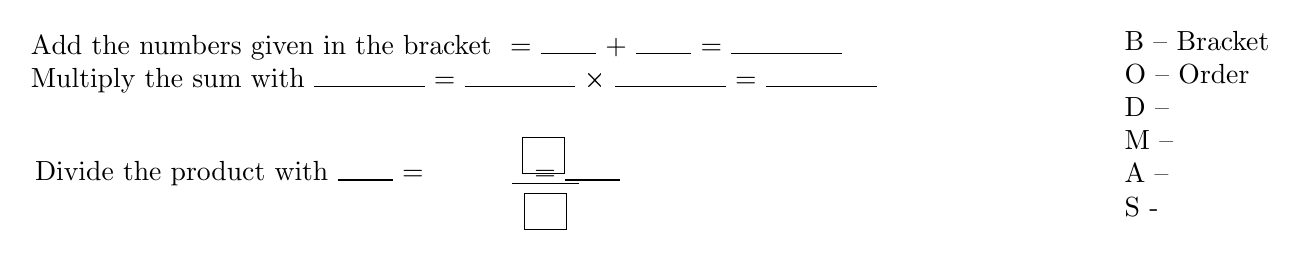
\begin{tikzpicture}[x=0.75pt,y=0.75pt,yscale=-1,xscale=1]



\draw    (242,96.67) -- (274.29,96.67) ;

\draw   (247,74.67) -- (267.29,74.67) -- (267.29,92.15) -- (247,92.15) -- cycle ;

\draw   (248,101.67) -- (268.29,101.67) -- (268.29,119.15) -- (248,119.15) -- cycle ;



\draw (9,24) node [anchor=north west][inner sep=0.75pt]   [align=left] {Add the numbers given in the bracket \ = \rule{20pt}{0.5pt} + \rule{20pt}{0.5pt} = \rule{40pt}{0.5pt}\\Multiply the sum with \rule{40pt}{0.5pt} = \rule{40pt}{0.5pt} × \rule{40pt}{0.5pt} = \rule{40pt}{0.5pt}\\\\};

\draw (11,85) node [anchor=north west][inner sep=0.75pt]   [align=left] {Divide the product with \rule{20pt}{0.5pt} = \ \ \ \ \ \ \ \ \ \ \ = \rule{20pt}{0.5pt}\\};

\draw (536,22) node [anchor=north west][inner sep=0.75pt]   [align=left] {B – Bracket\\O – Order\\D – \\M – \\A – \\S - \\};


\end{tikzpicture}
}%
\questionID {C6MDT23A}%
\question
{Answer the following questions.\bigskip{}

\tikzset{every picture/.style={line width=0.75pt}}         

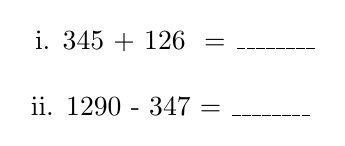
\begin{tikzpicture}[x=0.75pt,y=0.75pt,yscale=-1,xscale=1]


\draw (53,27) node [anchor=north west][inner sep=0.75pt]   [align=left] {i. 345 + 126 \ = \_\_\_\_\_\_\_\_};

\draw (51,59) node [anchor=north west][inner sep=0.75pt]   [align=left] {ii. 1290 - 347 = \_\_\_\_\_\_\_\_};


\end{tikzpicture}}%
\hints{\bigskip{}



\tikzset{every picture/.style={line width=0.75pt}}         

\begin{tikzpicture}[x=0.75pt,y=0.75pt,yscale=-1,xscale=1]


\draw    (357,210.02) -- (529,211.02) ;

\draw    (357,239.02) -- (527,239.02) ;

\draw    (125,207.02) -- (262,208.02) ;

\draw    (124,235.02) -- (261,236.02) ;




\draw (109,178) node [anchor=north west][inner sep=0.75pt]   [align=left] {(+)};

\draw (239,182) node [anchor=north west][inner sep=0.75pt]   [align=left] {6};

\draw (194,182) node [anchor=north west][inner sep=0.75pt]   [align=left] {2};

\draw (140,181) node [anchor=north west][inner sep=0.75pt]   [align=left] {1};

\draw (240,149) node [anchor=north west][inner sep=0.75pt]   [align=left] {5};

\draw (192,150) node [anchor=north west][inner sep=0.75pt]   [align=left] {4};

\draw (142,149) node [anchor=north west][inner sep=0.75pt]   [align=left] {3};

\draw (409,152) node [anchor=north west][inner sep=0.75pt]   [align=left] {2};

\draw (459,153) node [anchor=north west][inner sep=0.75pt]   [align=left] {9};

\draw (507,152) node [anchor=north west][inner sep=0.75pt]   [align=left] {0};

\draw (407,184) node [anchor=north west][inner sep=0.75pt]   [align=left] {3};

\draw (461,185) node [anchor=north west][inner sep=0.75pt]   [align=left] {4};

\draw (506,185) node [anchor=north west][inner sep=0.75pt]   [align=left] {7};

\draw (346,179) node [anchor=north west][inner sep=0.75pt]   [align=left] {(-)};

\draw (369,152) node [anchor=north west][inner sep=0.75pt]   [align=left] {1};


\end{tikzpicture}}%
\questionID {C6MDT23B}%
\question
{Fill in the blanks with correct symbol.( $>$ or $<$ or $=$ )


\tikzset{every picture/.style={line width=0.75pt}} 
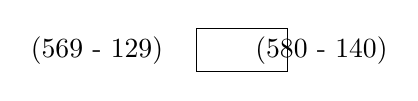
\begin{tikzpicture}[x=0.75pt,y=0.75pt,yscale=-1,xscale=1]


\draw   (203,126) -- (247,126) -- (247,147) -- (203,147) -- cycle ;



\draw (122,129) node [anchor=north west][inner sep=0.75pt]   [align=left] {(569 - 129) \ \ \ \ \ \ \ \ \  (580 - 140)};


\end{tikzpicture}}%
\hints{\bigskip{}

\tikzset{every picture/.style={line width=0.75pt}}        

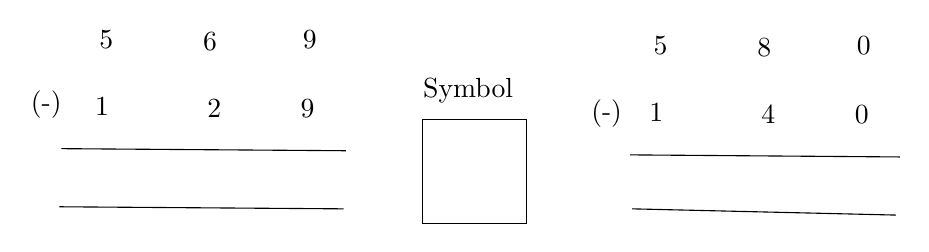
\begin{tikzpicture}[x=0.75pt,y=0.75pt,yscale=-1,xscale=1]


 
\draw    (419,230.02) -- (549,231.02) ;

\draw    (420,256.02) -- (547,259.02) ;

\draw    (145,227.02) -- (282,228.02) ;

\draw    (144,255.02) -- (281,256.02) ;


\draw   (319,213) -- (369,213) -- (369,263) -- (319,263) -- cycle ;



\draw (129,198) node [anchor=north west][inner sep=0.75pt]   [align=left] {(-)};

\draw (259,202) node [anchor=north west][inner sep=0.75pt]   [align=left] {9};

\draw (214,202) node [anchor=north west][inner sep=0.75pt]   [align=left] {2};

\draw (160,201) node [anchor=north west][inner sep=0.75pt]   [align=left] {1};

\draw (260,169) node [anchor=north west][inner sep=0.75pt]   [align=left] {9};

\draw (212,170) node [anchor=north west][inner sep=0.75pt]   [align=left] {6};

\draw (162,169) node [anchor=north west][inner sep=0.75pt]   [align=left] {5};

\draw (429,172) node [anchor=north west][inner sep=0.75pt]   [align=left] {5};

\draw (479,173) node [anchor=north west][inner sep=0.75pt]   [align=left] {8};

\draw (527,172) node [anchor=north west][inner sep=0.75pt]   [align=left] {0};

\draw (427,204) node [anchor=north west][inner sep=0.75pt]   [align=left] {1};

\draw (481,205) node [anchor=north west][inner sep=0.75pt]   [align=left] {4};

\draw (526,205) node [anchor=north west][inner sep=0.75pt]   [align=left] {0};

\draw (399,202) node [anchor=north west][inner sep=0.75pt]   [align=left] {(-)};

\draw (318,192) node [anchor=north west][inner sep=0.75pt]   [align=left] {Symbol};


\end{tikzpicture}}%
\questionID {C6MDT23C}%
\question
{In a village there are 6453 villagers, in which 1967 are women, 1509 children and remaining are the men. Find the number of men in the village ?}%
\hints{
\begin{align*}
 \text{Total number of villagers}  &= \rule{40pt}{0.5pt}\\
  \text{Number of women}  &= \rule{40pt}{0.5pt} \\
  \text{Number of children}  &= \rule{40pt}{0.5pt} \\
  \text{Number of men}  &= ( \rule{40pt}{0.5pt} )\quad – \quad ( \rule{40pt}{0.5pt} + \rule{40pt}{0.5pt} ) = \rule{40pt}{0.5pt}\\
\end{align*}

}%
\noindent\rule{\textwidth}{2pt}%
\linebreak%
\centering%
\begin{Large}%
\textbf{Data Handling}%
\end{Large}%
\linebreak%
\noindent\rule{\textwidth}{2pt}%
\begin{center}%
\medskip%
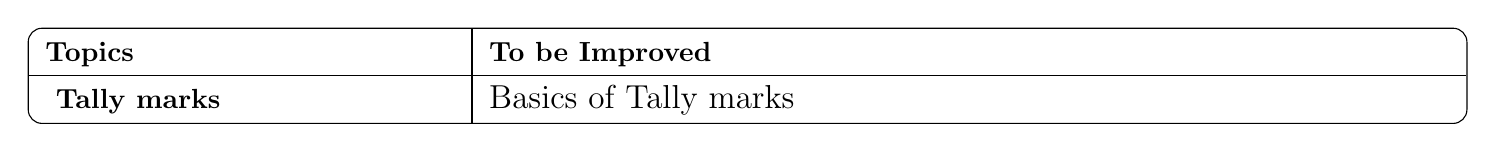
\begin{tikzpicture}%
\node (table) [inner sep=0pt] {%
{\renewcommand{\arraystretch}{1.4}%
\begin{tabular}{  m{5.2cm} | m{12.2cm}  } %
\textbf{Topics} & \textbf{To be Improved}
        \\
        \hline%
\normalsize{\textbf{ Tally marks}} & \large{Basics of Tally marks}%
\end{tabular}}};%
\draw [rounded corners=.5em] (table.north west) rectangle (table.south east);%
\end{tikzpicture}%
\end{center}%
\questionID {C6MDT38A}%
\question
{The fifth mark in a group of five marks should be used as a cross, as shown by

\tikzset{every picture/.style={line width=0.75pt}}        

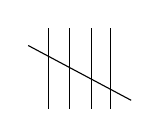
\begin{tikzpicture}[x=0.75pt,y=0.75pt,yscale=-1,xscale=1]



\draw    (147.87,115.2) -- (147.87,153.94) ;

\draw    (137.93,123.53) -- (187.53,149.93) ;

\draw    (157.87,115.2) -- (157.87,153.94) ;

\draw    (168.27,115.2) -- (168.27,153.94) ;

\draw    (177.47,115.2) -- (177.47,153.94) ;





\end{tikzpicture}
\\These are called \rule{80pt}{0.5pt}}%
\hints{A \rule{80pt}{0.5pt} is a collection of numbers gathered to give some information.\\
\bigskip
\tikzset{every picture/.style={line width=0.75pt}}        

\begin{tikzpicture}[x=0.75pt,y=0.75pt,yscale=-1,xscale=1]


\draw    (9.87,144.2) -- (9.87,182.94) ;

\draw    (-0.07,152.53) -- (49.53,178.93) ;

\draw    (19.87,144.2) -- (19.87,182.94) ;

\draw    (30.27,144.2) -- (30.27,182.94) ;

\draw    (39.47,144.2) -- (39.47,182.94) ;


\draw    (363.2,83.53) -- (363.2,122.27) ;

\draw    (373.2,83.53) -- (373.2,122.27) ;

\draw    (383.6,83.53) -- (383.6,122.27) ;

\draw    (392.8,83.53) -- (392.8,122.27) ;

\draw    (6.53,84.2) -- (6.53,122.94) ;

\draw    (16.53,84.2) -- (16.53,122.94) ;

\draw    (26.93,84.2) -- (26.93,122.94) ;

\draw    (363.2,32.87) -- (363.2,71.61) ;

\draw    (373.6,32.87) -- (373.6,71.61) ;

\draw    (6.93,32.87) -- (6.93,71.61) ;

\draw    (59.33,162.33) -- (92,162.33) ;
\draw [shift={(95,162.33)}, rotate = 180] [fill={rgb, 255:red, 0; green, 0; blue, 0 }  ][line width=0.08]  [draw opacity=0] (8.93,-4.29) -- (0,0) -- (8.93,4.29) -- cycle    ;

\draw    (409.67,105.67) -- (460.67,105.67) ;
\draw [shift={(463.67,105.67)}, rotate = 180] [fill={rgb, 255:red, 0; green, 0; blue, 0 }  ][line width=0.08]  [draw opacity=0] (8.93,-4.29) -- (0,0) -- (8.93,4.29) -- cycle    ;

\draw    (48,108.33) -- (92,108.33) ;
\draw [shift={(95,108.33)}, rotate = 180] [fill={rgb, 255:red, 0; green, 0; blue, 0 }  ][line width=0.08]  [draw opacity=0] (8.93,-4.29) -- (0,0) -- (8.93,4.29) -- cycle    ;

\draw    (396.67,53) -- (460.67,53) ;
\draw [shift={(463.67,53)}, rotate = 180] [fill={rgb, 255:red, 0; green, 0; blue, 0 }  ][line width=0.08]  [draw opacity=0] (8.93,-4.29) -- (0,0) -- (8.93,4.29) -- cycle    ;

\draw    (28,56) -- (92,56) ;
\draw [shift={(95,56)}, rotate = 180] [fill={rgb, 255:red, 0; green, 0; blue, 0 }  ][line width=0.08]  [draw opacity=0] (8.93,-4.29) -- (0,0) -- (8.93,4.29) -- cycle    ;


\draw (113.13,151.67) node [anchor=north west][inner sep=0.75pt]   [align=left] {represents = \rule{80pt}{0.5pt}};

\draw (477.67,95.67) node [anchor=north west][inner sep=0.75pt]   [align=left] {represents = \rule{80pt}{0.5pt}};

\draw (113.13,99) node [anchor=north west][inner sep=0.75pt]   [align=left] {represents = \rule{80pt}{0.5pt}};

\draw (477.67,43) node [anchor=north west][inner sep=0.75pt]   [align=left] {represents = \rule{80pt}{0.5pt}};

\draw (113.13,46) node [anchor=north west][inner sep=0.75pt]   [align=left] {represents = \rule{80pt}{0.5pt}};


\end{tikzpicture}\\


}%
\questionID {C6MDT38B}%
\question
{There are 12 students in a class. Represent this with tally marks.}%
\hints{Tally marks for 1 - \rule{40pt}{0.5pt}, 2 - \rule{40pt}{0.5pt}, 3 - \rule{40pt}{0.5pt}, 4 - \rule{40pt}{0.5pt}, 5 - \rule{40pt}{0.5pt}.\\
There are \rule{40pt}{0.5pt} students in the class. \\
In tally marks it is represented as \rule{40pt}{0.5pt}





}%
\questionID {C6MDT38C}%
\question
{ Fill the tally marks for the number of vehicles in an apartment.\begin{table}[H]
  \centering
\renewcommand{\arraystretch}{1.15}
    \begin{tabular}{|p{4.5cm}|p{3.5cm}|p{5.5cm}|}
    \hline
         Vehicles  & Tally Marks & Number of vehicles  \\
        \hline
         Cycle &   &10  \\
        \hline
         Bike &   & 18  \\
        \hline
         Car&    & 14  \\
        \hline
         \end{tabular}
\end{table}}%
\hints{
There are \rule{80pt}{0.5pt} cycles. Tally mark = \rule{80pt}{0.5pt}\\
There are \rule{80pt}{0.5pt} bikes. Tally mark = \rule{80pt}{0.5pt}\\
There are \rule{80pt}{0.5pt} cars. Tally mark =\rule{80pt}{0.5pt} }%
\noindent\rule{\textwidth}{2pt}%
\linebreak%
\centering%
\begin{Large}%
\textbf{Geometry}%
\end{Large}%
\linebreak%
\noindent\rule{\textwidth}{2pt}%
\begin{center}%
\medskip%
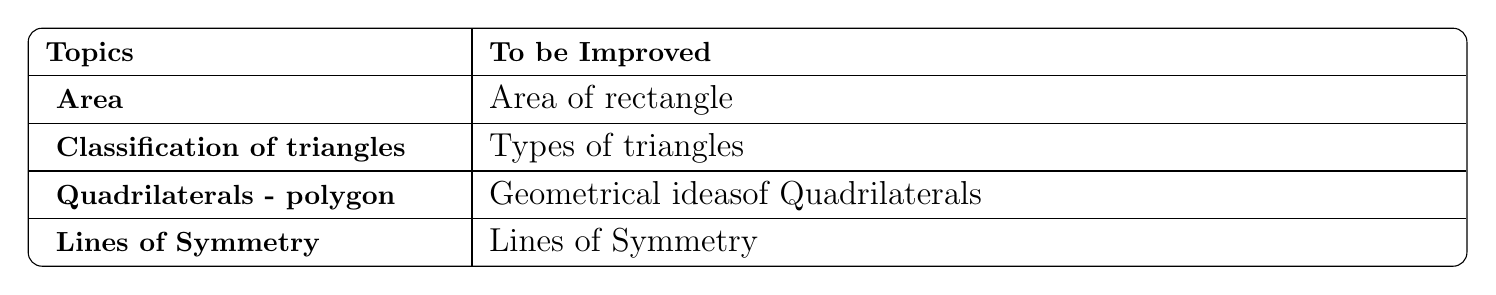
\begin{tikzpicture}%
\node (table) [inner sep=0pt] {%
{\renewcommand{\arraystretch}{1.4}%
\begin{tabular}{  m{5.2cm} | m{12.2cm}  } %
\textbf{Topics} & \textbf{To be Improved}
        \\
        \hline%
\normalsize{ \textbf{ Area}} & \large{Area of rectangle}%
\\
            \hline%
\normalsize{ \textbf{ Classification of triangles}} & \large{Types of triangles}%
\\
            \hline%
\normalsize{ \textbf{ Quadrilaterals - polygon}} & \large{Geometrical ideasof Quadrilaterals}%
\\
            \hline%
\normalsize{\textbf{ Lines of Symmetry}} & \large{Lines of Symmetry}%
\end{tabular}}};%
\draw [rounded corners=.5em] (table.north west) rectangle (table.south east);%
\end{tikzpicture}%
\end{center}%
\questionID {C6MDT29A}%
\question
{
What is the area of this rectangle ?
\begin{center}
    


\tikzset{every picture/.style={line width=0.75pt}}
\centering
\begin{tikzpicture}[x=0.75pt,y=0.75pt,yscale=-1,xscale=1]
\draw   (46,58) -- (203.8,58) -- (203.8,129) -- (46,129) -- cycle ;
\draw (106,139) node [anchor=north west][inner sep=0.75pt]   [align=left] {5 cm};
\draw (105,34) node [anchor=north west][inner sep=0.75pt]   [align=left] {5 cm};
\draw (213,83) node [anchor=north west][inner sep=0.75pt]   [align=left] {2 cm};
\draw (6,84) node [anchor=north west][inner sep=0.75pt]   [align=left] {2 cm};
\end{tikzpicture}
\end{center}
}%
\hints{{
\begin{align*}
 \text{Length of the rectangle}  &= \rule{160pt}{0.5pt}\\
 \text{Breadth of the rectangle}  &= \rule{160pt}{0.5pt}\\
 \text{Area of the rectangle}  &= \rule{40pt}{0.5pt}\hspace{5mm} \text{x} \hspace{5mm} \rule{80pt}{0.5pt}\\
  &= \rule{40pt}{0.5pt}\hspace{5mm} \text{x} \hspace{5mm} \rule{40pt}{0.5pt}\\
  \text{Area of the rectangle}  &= \rule{160pt}{0.5pt} \hspace{1mm} cm^{2} \\
\end{align*}
}}%
\questionID {C6MDT29B}%
\question
{

    
Which of the following rectangle has an area equivalent to 280 sq. m.\\
\begin{center}
\tikzset{every picture/.style={line width=0.75pt}}         

\begin{tikzpicture}[x=0.75pt,y=0.75pt,yscale=-1,xscale=1]

\draw   (107,78) -- (317.29,78) -- (317.29,178.35) -- (107,178.35) -- cycle ;

\draw   (441.65,67) -- (553,67) -- (553,178.35) -- (441.65,178.35) -- cycle ;


\draw (187,184) node [anchor=north west][inner sep=0.75pt]   [align=left] {24m};

\draw (67,123) node [anchor=north west][inner sep=0.75pt]   [align=left] {12m};

\draw (478,185) node [anchor=north west][inner sep=0.75pt]   [align=left] {20m};

\draw (407,105) node [anchor=north west][inner sep=0.75pt]   [align=left] {14m};

\draw (190,202) node [anchor=north west][inner sep=0.75pt]   [align=left] {(i)};

\draw (487,204) node [anchor=north west][inner sep=0.75pt]   [align=left] {(ii)};


\end{tikzpicture}
\end{center}

}%
\hints{Rectangle (i)
\begin{align*}
 \text{Length of the rectangle}  &= \rule{160pt}{0.5pt}\\
 \text{Breadth of the rectangle}  &= \rule{160pt}{0.5pt}\\
 \text{Area of the rectangle}  &= \rule{80pt}{0.5pt} \hspace{5mm} \text{x} \hspace{5mm} \rule{80pt}{0.5pt}\\
  &= \rule{80pt}{0.5pt}\hspace{5mm} \text{x} \hspace{5mm} \rule{80pt}{0.5pt}\\
  \text{Area of the rectangle}  &= \rule{160pt}{0.5pt} \hspace{1mm} 
 (=/ \neq) \quad 280 \text { sq.m }\\
\end{align*}\\
Rectangle (ii)
\begin{align*}
 \text{Length of the rectangle}  &= \rule{160pt}{0.5pt}\\
 \text{Breadth of the rectangle}  &= \rule{160pt}{0.5pt}\\
 \text{Area of the rectangle}  &= \rule{40pt}{0.5pt} \hspace{5mm} \text{x} \hspace{5mm} \rule{40pt}{0.5pt}\\
  &= \rule{40pt}{0.5pt}\hspace{5mm} \text{x} \hspace{5mm} \rule{40pt}{0.5pt}\\
  \text{Area of the rectangle}  &= \rule{160pt}{0.5pt} \hspace{1mm} 
 (=/ \neq) \quad 280 \text { sq.m }\\
\end{align*}
}%
\questionID {C6MDT29C}%
\question
{Area of a rectangular street is 2640m² and its length = 44m . What is the breadth of the street?}%
\hints{\begin{align*}
 \text{Length of the rectangle street}  &= \rule{160pt}{0.5pt}\\
 \text{Breadth of the rectangle street}  &= \rule{160pt}{0.5pt}\\
 \text{Area of the rectangle}  &= \rule{80pt}{0.5pt} \hspace{5mm} \text{x} \hspace{5mm} \rule{80pt}{0.5pt} cm ^{2}\end{align*}\\

\begin{center}
\tikzset{every picture/.style={line width=0.75pt}}
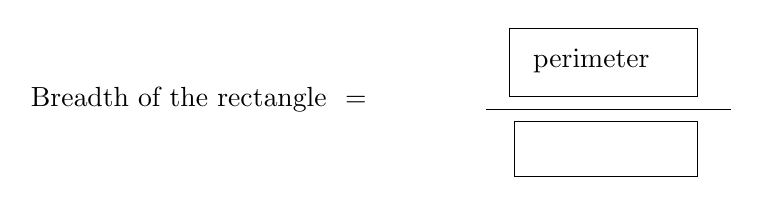
\begin{tikzpicture}[x=0.75pt,y=0.75pt,yscale=-1,xscale=1]
\draw    (306,63.05) -- (424,63.05) ;
\draw   (320.05,68.87) -- (408,68.87) -- (408,95.47) -- (320.05,95.47) -- cycle ;
\draw   (317.58,24.05) -- (408,24.05) -- (408,56.92) -- (317.58,56.92) -- cycle ;
\draw (85.6,51.16) node [anchor=north west][inner sep=0.75pt]   [align=left] {Breadth of the rectangle \ =};
\draw (327.64,32.73) node [anchor=north west][inner sep=0.75pt]   [align=left] {perimeter};
\end{tikzpicture}\\
Breadth of the rectangular street $=$ 
\end{center}
}%
\questionID {C6MDT36A}%
\question
{Which of the following triangle is a right-angled triangle ? \\

\begin{center}
\tikzset{every picture/.style={line width=0.75pt}} 
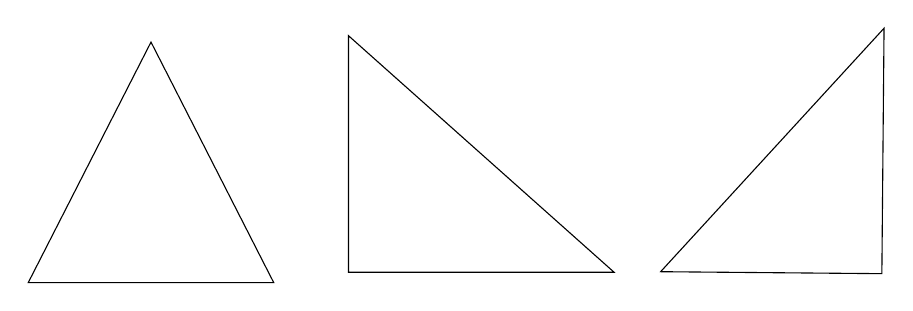
\begin{tikzpicture}[x=0.75pt,y=0.75pt,yscale=-1,xscale=1]

\draw   (125.75,67.4) -- (184.89,183.32) -- (66.6,183.32) -- cycle ;
\draw   (220.89,64.32) -- (348.89,178.32) -- (220.89,178.32) -- cycle ;
\draw   (371.29,178.03) -- (478.93,60.73) -- (477.88,178.98) -- cycle ;

\end{tikzpicture}
\end{center}
}%
\hints{The angle made at the right angle  is \rule{80pt}{0.5pt}°\\
A triangle with right angle is called as \rule{80pt}{0.5pt}.\\
}%
\questionID {C6MDT36B}%
\question
{Draw an example of\\
\begin{enumerate}
    \item Scalene triangle\\ 
    \item Obtuse angled triangle\\
    \item Equilateral triangle \\
\end{enumerate}}%
\hints{The sides and angle are different in \rule{80pt}{0.5pt} triangle.\\
All the sides and angles are equal in \rule{80pt}{0.5pt} triangle.\\
If one of the angle is greater than 90°, then the triangle is called as \rule{80pt}{0.5pt}.}%
\questionID {C6MDT36C}%
\question
{Name each of the following triangles in two different ways (based on angles and based on sides).\\ \bigskip

\tikzset{every picture/.style={line width=0.75pt}}        

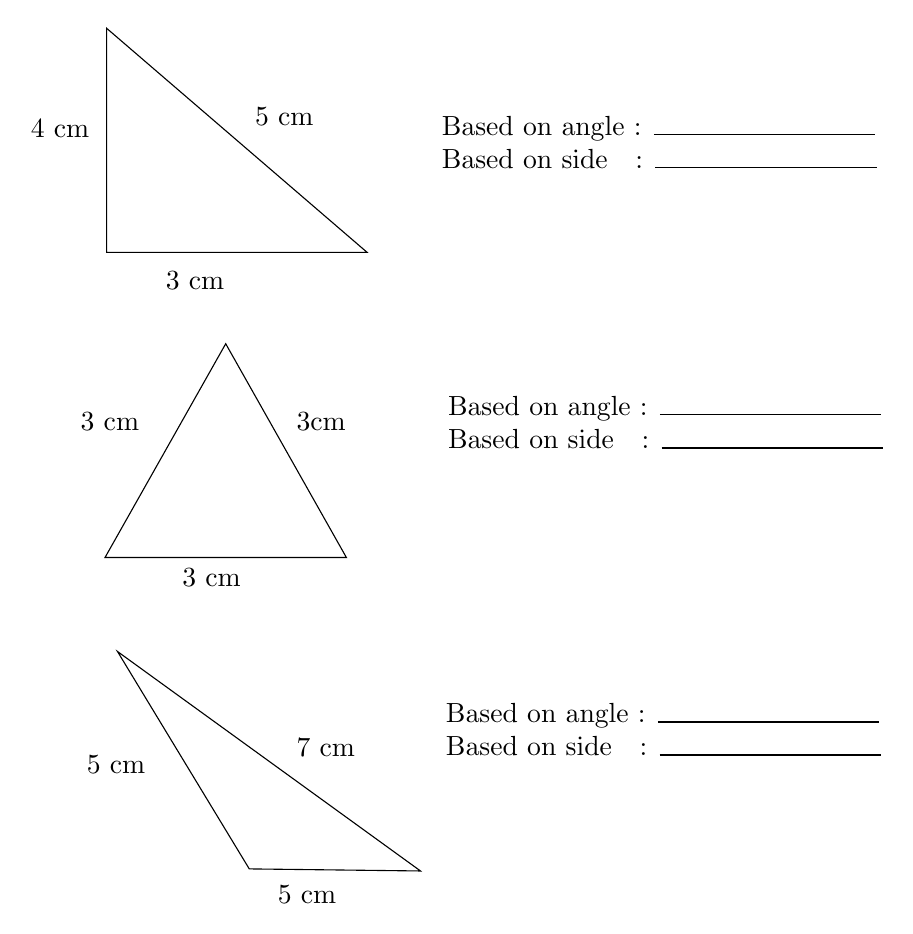
\begin{tikzpicture}[x=0.75pt,y=0.75pt,yscale=-1,xscale=1]

\draw   (91.75,18.99) -- (217.29,126.99) -- (91.75,126.99) -- cycle ;

\draw   (149.15,171) -- (207.29,273.99) -- (91,273.99) -- cycle ;

\draw   (243,425.02) -- (160.5,424.02) -- (97,319.27) -- (141.43,351.45) -- (141.53,351.52) -- (158.88,364.09) -- cycle ;



\draw (252,60) node [anchor=north west][inner sep=0.75pt]   [align=left] {Based on angle : \rule{80pt}{0.5pt}\\Based on side \ \ : \rule{80pt}{0.5pt}};
\draw (255,195) node [anchor=north west][inner sep=0.75pt]   [align=left] {Based on angle : \rule{80pt}{0.5pt}\\Based on side \ \ : \rule{80pt}{0.5pt}};

\draw (254,343) node [anchor=north west][inner sep=0.75pt]   [align=left] {Based on angle : \rule{80pt}{0.5pt}\\Based on side \ \ : \rule{80pt}{0.5pt}};

\draw (162,56) node [anchor=north west][inner sep=0.75pt]   [align=left] {5 cm};

\draw (54,62) node [anchor=north west][inner sep=0.75pt]   [align=left] {4 cm};

\draw (119,135) node [anchor=north west][inner sep=0.75pt]   [align=left] {3 cm};

\draw (78,203) node [anchor=north west][inner sep=0.75pt]   [align=left] {3 cm};

\draw (127,278) node [anchor=north west][inner sep=0.75pt]   [align=left] {3 cm};

\draw (182,203) node [anchor=north west][inner sep=0.75pt]   [align=left] {3cm};

\draw (81,368) node [anchor=north west][inner sep=0.75pt]   [align=left] {5 cm};

\draw (173,431) node [anchor=north west][inner sep=0.75pt]   [align=left] {5 cm};

\draw (182,360) node [anchor=north west][inner sep=0.75pt]   [align=left] {7 cm};
\end{tikzpicture}\\ \bigskip}%
\hints{
A triangle having all three unequal sides is called a \rule{80pt}{0.5pt}.\\
A triangle having three equal sides is called an \rule{80pt}{0.5pt}.\\
A triangle having two equal sides is called an \rule{80pt}{0.5pt}.\\
If each angle is less than 90°, then the triangle is called an \rule{80pt}{0.5pt}.\\
If any one angle is a right angle then the triangle is called a \rule{80pt}{0.5pt}.\\
If any one angle is greater than 90°, then the triangle is called an \rule{80pt}{0.5pt}.
}%
\questionID {C6MDT33A}%
\question
{Any two sides with a common end point are called the \rule{80pt}{0.5pt} sides of the polygon.}%
\hints{ 
\rule{80pt}{0.5pt} is closed figure with 3 or more sides.\\

\begin{center}
 Mark the adjacent angles.\bigskip   

\tikzset{every picture/.style={line width=0.75pt}}

\begin{tikzpicture}[x=0.75pt,y=0.75pt,yscale=-1,xscale=1]


\draw   (140,134.05) -- (284,134.05) -- (284,191.05) -- (140,191.05) -- cycle ;


\draw (125,121.05) node [anchor=north west][inner sep=0.75pt]   [align=left] {A};

\draw (288,123.05) node [anchor=north west][inner sep=0.75pt]   [align=left] {B};

\draw (286,189.05) node [anchor=north west][inner sep=0.75pt]   [align=left] {C};

\draw (125,188.05) node [anchor=north west][inner sep=0.75pt]   [align=left] {D};


\end{tikzpicture}\end{center}

Any two sides with a common end point are called the  \rule{80pt}{0.5pt} sides of the polygon.
}%
\questionID {C6MDT33B}%
\question
{Name the diagonals from the given figure. \\
\bigskip{}
\begin{center}
    

\tikzset{every picture/.style={line width=0.75pt}} 
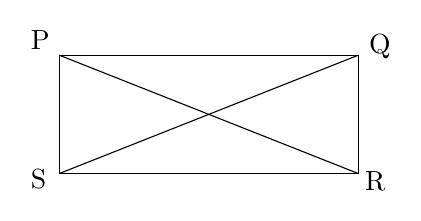
\begin{tikzpicture}[x=0.75pt,y=0.75pt,yscale=-1,xscale=1]



\draw   (120,114.05) -- (264,114.05) -- (264,171.05) -- (120,171.05) -- cycle ;

\draw    (120,114.05) -- (264,171.05) ;

\draw    (120,171.05) -- (264,114.05) ;



\draw (105,101.05) node [anchor=north west][inner sep=0.75pt]   [align=left] {P};

\draw (268,103.05) node [anchor=north west][inner sep=0.75pt]   [align=left] {Q};

\draw (266,169.05) node [anchor=north west][inner sep=0.75pt]   [align=left] {R};

\draw (105,168.05) node [anchor=north west][inner sep=0.75pt]   [align=left] {S};


\end{tikzpicture}\end{center}}%
\hints{A \rule{80pt}{0.5pt} is a straight line connecting the opposite corners of a polygon through its vertex .\\
The given figure PQRS is a \rule{80pt}{0.5pt}\\
The sides of the given shape are \rule{40pt}{0.5pt}\\
The diagonals in the given figure is \rule{40pt}{0.5pt}
}%
\questionID {C6MDT33C}%
\question
{Mark the sides, diagonals and adjacent sides in the rhombus.\\
\begin{center}
    

\tikzset{every picture/.style={line width=0.75pt}} 
\begin{tikzpicture}[x=0.75pt,y=0.75pt,yscale=-1,xscale=1]


\draw   (139.5,107) -- (179,146.5) -- (139.5,186) -- (100,146.5) -- cycle ;


\draw (134,88) node [anchor=north west][inner sep=0.75pt]   [align=left] {A};

\draw (185,139) node [anchor=north west][inner sep=0.75pt]   [align=left] {B};

\draw (135,188) node [anchor=north west][inner sep=0.75pt]   [align=left] {C};

\draw (83,137) node [anchor=north west][inner sep=0.75pt]   [align=left] {D};


\end{tikzpicture}\end{center}}%
\hints{The given shape is \rule{80pt}{0.5pt}. \\
The sides of the polygon is \rule{80pt}{0.5pt}. \\
The diagonals of the polygon is \rule{80pt}{0.5pt}. \\
The adjacent sides of the polygon is \rule{80pt}{0.5pt}.
}%
\questionID {C6MDT26A}%
\question
{Draw the line of symmetry for this shape.\\
\begin{center}
\tikzset{every picture/.style={line width=0.75pt}} 


\begin{tikzpicture}[x=0.75pt,y=0.75pt,yscale=-1,xscale=1]


\draw   (220,98.01) .. controls (220,69.85) and (242.83,47.02) .. (270.99,47.02) .. controls (299.15,47.02) and (321.98,69.85) .. (321.98,98.01) .. controls (321.98,126.17) and (299.15,149) .. (270.99,149) .. controls (242.83,149) and (220,126.17) .. (220,98.01) -- cycle ;

\draw   (281.98,89.51) .. controls (281.98,84.81) and (285.79,81) .. (290.49,81) .. controls (295.19,81) and (299,84.81) .. (299,89.51) .. controls (299,94.21) and (295.19,98.02) .. (290.49,98.02) .. controls (285.79,98.02) and (281.98,94.21) .. (281.98,89.51) -- cycle ;

\draw   (238.98,89.51) .. controls (238.98,84.81) and (242.79,81) .. (247.49,81) .. controls (252.19,81) and (256,84.81) .. (256,89.51) .. controls (256,94.21) and (252.19,98.02) .. (247.49,98.02) .. controls (242.79,98.02) and (238.98,94.21) .. (238.98,89.51) -- cycle ;

\draw  [draw opacity=0] (291.63,108.83) .. controls (293.23,111.02) and (294.19,113.51) .. (294.3,116.19) .. controls (294.69,125.48) and (284.77,133.44) .. (272.15,133.97) .. controls (259.54,134.5) and (248.99,127.39) .. (248.61,118.1) .. controls (248.49,115.42) and (249.24,112.85) .. (250.65,110.54) -- (271.45,117.14) -- cycle ; \draw   (291.63,108.83) .. controls (293.23,111.02) and (294.19,113.51) .. (294.3,116.19) .. controls (294.69,125.48) and (284.77,133.44) .. (272.15,133.97) .. controls (259.54,134.5) and (248.99,127.39) .. (248.61,118.1) .. controls (248.49,115.42) and (249.24,112.85) .. (250.65,110.54) ;  




\end{tikzpicture}
\end{center}}%
\hints{In symmetry if a image is divided by a line, that image should be divided into \rule{80pt}{0.5pt} symmetric parts.\\
Let’s assume a line X to find the symmetricity of the given figure, \\
The line X divides the image equally. Hence, X is the \rule{80pt}{0.5pt}.}%
\questionID {C6MDT26B}%
\question
{ \rule{80pt}{0.5pt} lines of symmetry can be drawn for a hexagon ?}%
\hints{The line of symmetry is also called as \rule{80pt}{0.5pt}.\\A hexagon has \rule{80pt}{0.5pt} sides.\\
Mark the lines of symmetry.\\
\begin{center}
    
\bigskip

\tikzset{every picture/.style={line width=0.75pt}}     

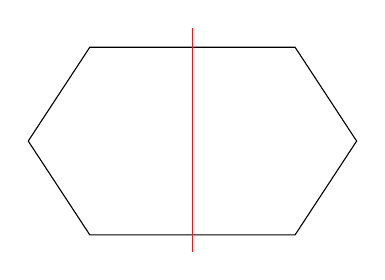
\begin{tikzpicture}[x=0.75pt,y=0.75pt,yscale=-1,xscale=1]


\draw   (180,126.36) -- (209.67,81.15) -- (308.56,81.15) -- (338.23,126.36) -- (308.56,171.57) -- (209.67,171.57) -- cycle ;
 
\draw [color={rgb, 255:red, 230; green, 27; blue, 27 }  ,draw opacity=1 ]   (259,72) -- (259,179.57) ;
\end{tikzpicture}\\
\end{center}
\bigskip
Therefore, the hexagon has \rule{80pt}{0.5pt} lines of symmetry.}%
\questionID {C6MDT26C}%
\question
{


Draw the lines of symmetry for the following figures.\\


\begin{center}
\tikzset{every picture/.style={line width=0.75pt}}

\begin{tikzpicture}[x=0.75pt,y=0.75pt,yscale=-1,xscale=1]



\draw   (111.65,117) -- (177.29,218.88) -- (46,218.88) -- cycle ;

\draw   (273.15,111.71) -- (327.29,165.85) -- (273.15,220) -- (219,165.85) -- cycle ;

\draw   (362.46,167.5) .. controls (362.46,139.61) and (385.06,117) .. (412.96,117) .. controls (440.85,117) and (463.46,139.61) .. (463.46,167.5) .. controls (463.46,195.39) and (440.85,218) .. (412.96,218) .. controls (385.06,218) and (362.46,195.39) .. (362.46,167.5) -- cycle ;





\end{tikzpicture}
\end{center}}%
\hints{\bigskip


\tikzset{every picture/.style={line width=0.75pt}}      \begin{tikzpicture}[x=0.75pt,y=0.75pt,yscale=-1,xscale=1]
\draw   (111.65,117) -- (177.29,218.88) -- (46,218.88) -- cycle ;
 
\draw   (273.15,111.71) -- (327.29,165.85) -- (273.15,220) -- (219,165.85) -- cycle ;

\draw   (362.46,167.5) .. controls (362.46,139.61) and (385.06,117) .. (412.96,117) .. controls (440.85,117) and (463.46,139.61) .. (463.46,167.5) .. controls (463.46,195.39) and (440.85,218) .. (412.96,218) .. controls (385.06,218) and (362.46,195.39) .. (362.46,167.5) -- cycle ;
\end{tikzpicture}\\ \bigskip

An image is said to be symmetrical if it has \rule{80pt}{0.5pt} balanced proportion.\\


\tikzset{every picture/.style={line width=0.75pt}}        

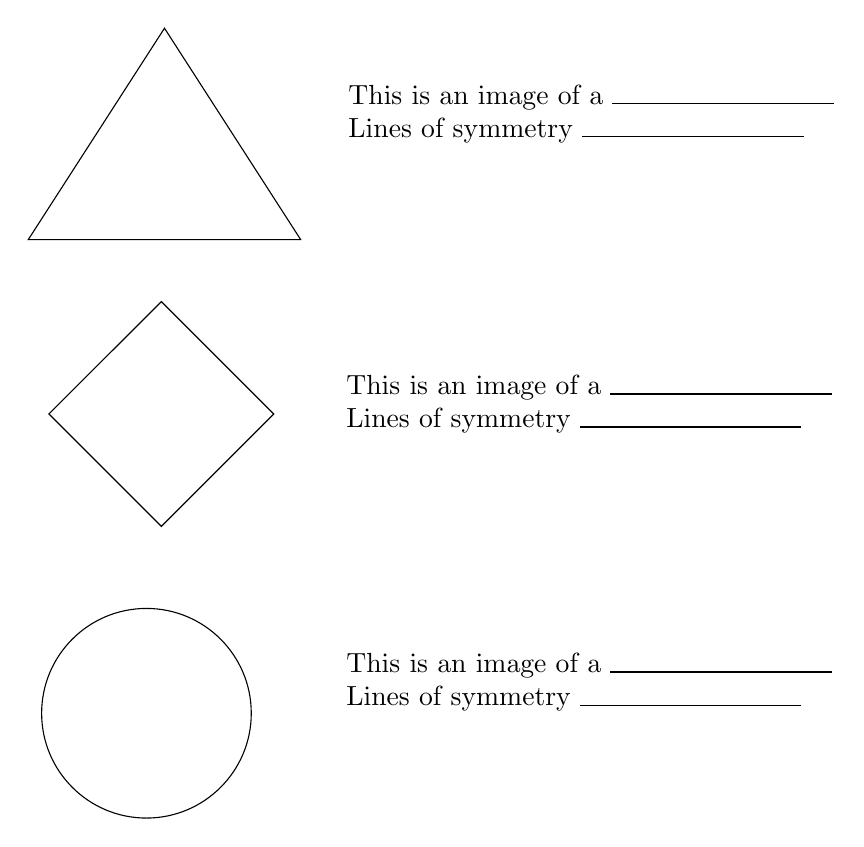
\begin{tikzpicture}[x=0.75pt,y=0.75pt,yscale=-1,xscale=1]
\draw   (95.65,25) -- (161.29,126.88) -- (30,126.88) -- cycle ;
 
\draw   (94.15,156.71) -- (148.29,210.85) -- (94.15,265) -- (40,210.85) -- cycle ;

\draw   (36.46,355.04) .. controls (36.46,327.15) and (59.06,304.54) .. (86.96,304.54) .. controls (114.85,304.54) and (137.46,327.15) .. (137.46,355.04) .. controls (137.46,382.94) and (114.85,405.54) .. (86.96,405.54) .. controls (59.06,405.54) and (36.46,382.94) .. (36.46,355.04) -- cycle ;



\draw (183,51) node [anchor=north west][inner sep=0.75pt]   [align=left] {This is an image of a \rule{80pt}{0.5pt}\\Lines of symmetry \rule{80pt}{0.5pt}};

\draw (182,191) node [anchor=north west][inner sep=0.75pt]   [align=left] {This is an image of a \rule{80pt}{0.5pt}\\Lines of symmetry \rule{80pt}{0.5pt}};

\draw (182,325) node [anchor=north west][inner sep=0.75pt]   [align=left] {This is an image of a \rule{80pt}{0.5pt}\\Lines of symmetry \rule{80pt}{0.5pt}};
\end{tikzpicture}
}%
\noindent\rule{\textwidth}{2pt}%
\linebreak%
\centering%
\begin{Large}%
\textbf{Number system}%
\end{Large}%
\linebreak%
\noindent\rule{\textwidth}{2pt}%
\begin{center}%
\medskip%
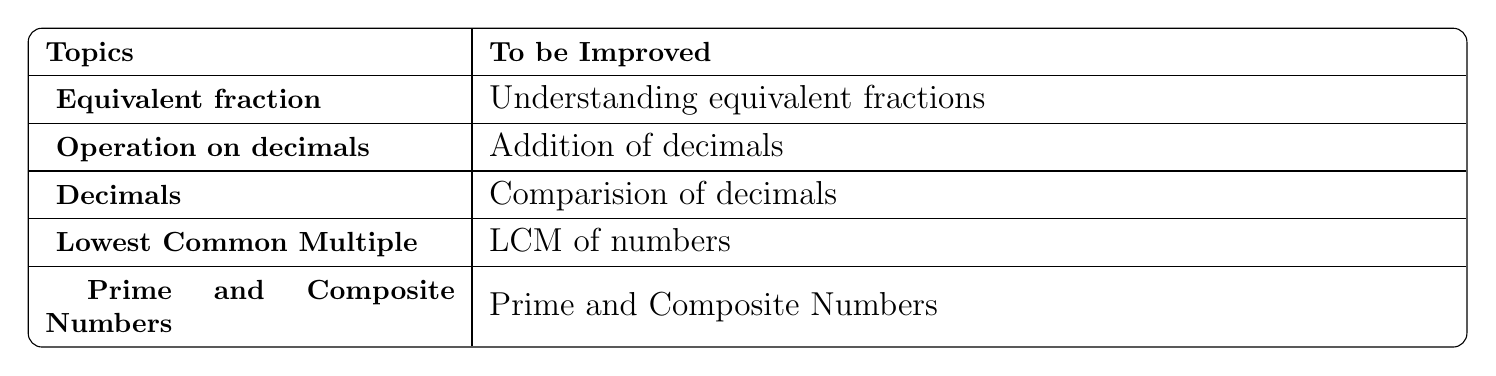
\begin{tikzpicture}%
\node (table) [inner sep=0pt] {%
{\renewcommand{\arraystretch}{1.4}%
\begin{tabular}{  m{5.2cm} | m{12.2cm}  } %
\textbf{Topics} & \textbf{To be Improved}
        \\
        \hline%
\normalsize{ \textbf{ Equivalent fraction}} & \large{Understanding equivalent fractions}%
\\
            \hline%
\normalsize{ \textbf{ Operation on decimals}} & \large{Addition of decimals}%
\\
            \hline%
\normalsize{ \textbf{ Decimals}} & \large{Comparision of decimals}%
\\
            \hline%
\normalsize{ \textbf{ Lowest Common Multiple}} & \large{LCM of numbers}%
\\
            \hline%
\normalsize{\textbf{ Prime and Composite Numbers}} & \large{Prime and Composite Numbers}%
\end{tabular}}};%
\draw [rounded corners=.5em] (table.north west) rectangle (table.south east);%
\end{tikzpicture}%
\end{center}%
\questionID {C6MDT7A}%
\question
{

\tikzset{every picture/.style={line width=0.75pt}} 
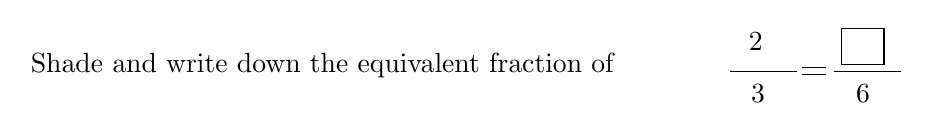
\begin{tikzpicture}[x=0.75pt,y=0.75pt,yscale=-1,xscale=1]



\draw    (393,65.67) -- (425.29,65.67) ;

\draw   (447,44.67) -- (467.29,44.67) -- (467.29,62.15) -- (447,62.15) -- cycle ;

\draw    (443,65.67) -- (475.29,65.67) ;

\draw    (428,63.67) -- (439.29,63.67) ;
 
\draw    (428,67.15) -- (439.29,67.15) ;





\draw (401,45.67) node [anchor=north west][inner sep=0.75pt]   [align=left] {2};

\draw (402,70.67) node [anchor=north west][inner sep=0.75pt]   [align=left] {3};

\draw (452.67,70.67) node [anchor=north west][inner sep=0.75pt]   [align=left] {6};

\draw (55,55.67) node [anchor=north west][inner sep=0.75pt]   [align=left] {Shade and write down the equivalent fraction of };


\end{tikzpicture}\\



  
\tikzset {_f36cnbrul/.code = {\pgfsetadditionalshadetransform{ \pgftransformshift{\pgfpoint{0 bp } { 0 bp }  }  \pgftransformrotate{0 }  \pgftransformscale{2 }  }}}
\pgfdeclarehorizontalshading{_0gr4zptg6}{150bp}{rgb(0bp)=(1,1,1);
rgb(37.5bp)=(1,1,1);
rgb(62.5bp)=(0,0,0);
rgb(100bp)=(0,0,0)}
\tikzset{_1m26lfijh/.code = {\pgfsetadditionalshadetransform{\pgftransformshift{\pgfpoint{0 bp } { 0 bp }  }  \pgftransformrotate{0 }  \pgftransformscale{2 } }}}
\pgfdeclarehorizontalshading{_3atre3ypt} {150bp} {color(0bp)=(transparent!0);
color(37.5bp)=(transparent!0);
color(62.5bp)=(transparent!10);
color(100bp)=(transparent!10) } 
\pgfdeclarefading{_qow1hqzsm}{\tikz \fill[shading=_3atre3ypt,_1m26lfijh] (0,0) rectangle (50bp,50bp); } 


  
\tikzset {_q6sayq8gc/.code = {\pgfsetadditionalshadetransform{ \pgftransformshift{\pgfpoint{0 bp } { 0 bp }  }  \pgftransformrotate{0 }  \pgftransformscale{2 }  }}}
\pgfdeclarehorizontalshading{_3m5nks3d9}{150bp}{rgb(0bp)=(1,1,1);
rgb(37.5bp)=(1,1,1);
rgb(62.5bp)=(0,0,0);
rgb(100bp)=(0,0,0)}
\tikzset{_35ww7fz1b/.code = {\pgfsetadditionalshadetransform{\pgftransformshift{\pgfpoint{0 bp } { 0 bp }  }  \pgftransformrotate{0 }  \pgftransformscale{2 } }}}
\pgfdeclarehorizontalshading{_1dbc0n4wn} {150bp} {color(0bp)=(transparent!0);
color(37.5bp)=(transparent!0);
color(62.5bp)=(transparent!10);
color(100bp)=(transparent!10) } 
\pgfdeclarefading{_eadpz6pf5}{\tikz \fill[shading=_1dbc0n4wn,_35ww7fz1b] (0,0) rectangle (50bp,50bp); } 
\tikzset{every picture/.style={line width=0.75pt}}       

\begin{tikzpicture}[x=0.75pt,y=0.75pt,yscale=-1,xscale=1]


\path  [shading=_0gr4zptg6,_f36cnbrul,path fading= _qow1hqzsm ,fading transform={xshift=2}] (31.67,63) -- (92.33,63) -- (92.33,127) -- (31.67,127) -- cycle ; 
 \draw  [color={rgb, 255:red, 0; green, 0; blue, 0 }  ,draw opacity=1 ] (31.67,63) -- (92.33,63) -- (92.33,127) -- (31.67,127) -- cycle ; 


\path  [shading=_3m5nks3d9,_q6sayq8gc,path fading= _eadpz6pf5 ,fading transform={xshift=2}] (92.33,63) -- (153,63) -- (153,127) -- (92.33,127) -- cycle ; 
 \draw   (92.33,63) -- (153,63) -- (153,127) -- (92.33,127) -- cycle ; 


\draw   (153,63) -- (213.67,63) -- (213.67,127) -- (153,127) -- cycle ;

\draw  [color={rgb, 255:red, 0; green, 0; blue, 0 }  ,draw opacity=1 ] (279,64) -- (339.67,64) -- (339.67,128) -- (279,128) -- cycle ;

\draw   (339.67,64) -- (400.33,64) -- (400.33,128) -- (339.67,128) -- cycle ;

\draw   (400.33,64) -- (461,64) -- (461,128) -- (400.33,128) -- cycle ;


\draw  [color={rgb, 255:red, 0; green, 0; blue, 0 }  ,draw opacity=1 ] (461,64) -- (521.67,64) -- (521.67,128) -- (461,128) -- cycle ;
 
\draw   (521.67,64) -- (582.33,64) -- (582.33,128) -- (521.67,128) -- cycle ;

\draw   (582.33,64) -- (643,64) -- (643,128) -- (582.33,128) -- cycle ;



\draw    (236,90) -- (253.67,90) ;

\draw    (236.67,96) -- (254.33,96) ;




\end{tikzpicture}

}%
\hints{

\bigskip  
\tikzset {_nf7tfw7gi/.code = {\pgfsetadditionalshadetransform{ \pgftransformshift{\pgfpoint{0 bp } { 0 bp }  }  \pgftransformrotate{0 }  \pgftransformscale{2 }  }}}
\pgfdeclarehorizontalshading{_z9d3vpu0x}{150bp}{rgb(0bp)=(1,1,1);
rgb(37.5bp)=(1,1,1);
rgb(62.5bp)=(0,0,0);
rgb(100bp)=(0,0,0)}
\tikzset{_prwtbkbh3/.code = {\pgfsetadditionalshadetransform{\pgftransformshift{\pgfpoint{0 bp } { 0 bp }  }  \pgftransformrotate{0 }  \pgftransformscale{2 } }}}
\pgfdeclarehorizontalshading{_njh1de96e} {150bp} {color(0bp)=(transparent!0);
color(37.5bp)=(transparent!0);
color(62.5bp)=(transparent!10);
color(100bp)=(transparent!10) } 
\pgfdeclarefading{_rraq0rpsm}{\tikz \fill[shading=_njh1de96e,_prwtbkbh3] (0,0) rectangle (50bp,50bp); } 


  
\tikzset {_1eb4930jl/.code = {\pgfsetadditionalshadetransform{ \pgftransformshift{\pgfpoint{0 bp } { 0 bp }  }  \pgftransformrotate{0 }  \pgftransformscale{2 }  }}}
\pgfdeclarehorizontalshading{_mcx9fjc81}{150bp}{rgb(0bp)=(1,1,1);
rgb(37.5bp)=(1,1,1);
rgb(62.5bp)=(0,0,0);
rgb(100bp)=(0,0,0)}
\tikzset{_9n83cbmhx/.code = {\pgfsetadditionalshadetransform{\pgftransformshift{\pgfpoint{0 bp } { 0 bp }  }  \pgftransformrotate{0 }  \pgftransformscale{2 } }}}
\pgfdeclarehorizontalshading{_b04l00aek} {150bp} {color(0bp)=(transparent!0);
color(37.5bp)=(transparent!0);
color(62.5bp)=(transparent!10);
color(100bp)=(transparent!10) } 
\pgfdeclarefading{_y5rztskdi}{\tikz \fill[shading=_b04l00aek,_9n83cbmhx] (0,0) rectangle (50bp,50bp); } 
\tikzset{every picture/.style={line width=0.75pt}} 
\begin{tikzpicture}[x=0.75pt,y=0.75pt,yscale=-1,xscale=1]


\path  [shading=_z9d3vpu0x,_nf7tfw7gi,path fading= _rraq0rpsm ,fading transform={xshift=2}] (12,61) -- (72.67,61) -- (72.67,125) -- (12,125) -- cycle ; 
 \draw  [color={rgb, 255:red, 0; green, 0; blue, 0 }  ,draw opacity=1 ] (12,61) -- (72.67,61) -- (72.67,125) -- (12,125) -- cycle ; 


\path  [shading=_mcx9fjc81,_1eb4930jl,path fading= _y5rztskdi ,fading transform={xshift=2}] (72.67,61) -- (133.33,61) -- (133.33,125) -- (72.67,125) -- cycle ; 
 \draw   (72.67,61) -- (133.33,61) -- (133.33,125) -- (72.67,125) -- cycle ;


\draw  [color={rgb, 255:red, 0; green, 0; blue, 0 }  ,draw opacity=1 ] (11,197) -- (71.67,197) -- (71.67,261) -- (11,261) -- cycle ;

\draw   (71.67,197) -- (132.33,197) -- (132.33,261) -- (71.67,261) -- cycle ;

\draw   (132.33,197) -- (193,197) -- (193,261) -- (132.33,261) -- cycle ;


\draw  [color={rgb, 255:red, 0; green, 0; blue, 0 }  ,draw opacity=1 ] (193,197) -- (253.67,197) -- (253.67,261) -- (193,261) -- cycle ;

\draw   (253.67,197) -- (314.33,197) -- (314.33,261) -- (253.67,261) -- cycle ;

\draw   (314.33,197) -- (375,197) -- (375,261) -- (314.33,261) -- cycle ;



\draw   (133.33,61) -- (194,61) -- (194,125) -- (133.33,125) -- cycle ;

\draw    (10.4,161) -- (29.5,161) ;

\draw   (64.4,140) -- (84.69,140) -- (84.69,157.48) -- (64.4,157.48) -- cycle ;

\draw   (114,140) -- (134.29,140) -- (134.29,157.48) -- (114,157.48) -- cycle ;


\draw   (64.4,164) -- (84.69,164) -- (84.69,181.48) -- (64.4,181.48) -- cycle ;

\draw   (114,164) -- (134.29,164) -- (134.29,181.48) -- (114,181.48) -- cycle ;

 
\draw    (60.4,161) -- (92.69,161) ;
 
\draw    (110,161) -- (142.29,161) ;
 
\draw    (95,159) -- (106.29,159) ;
 
\draw    (95,162.48) -- (106.29,162.48) ;



\draw (209,74) node [anchor=north west][inner sep=0.75pt]   [align=left] {There are \rule{40pt}{0.5pt} square boxes filled out of 3 square boxes.\\The fraction is \rule{40pt}{0.5pt}.};

\draw (168,154) node [anchor=north west][inner sep=0.75pt]   [align=left] {6 is twice of 3, \rule{40pt}{0.5pt} is twice of 2\\};

\draw (11,24) node [anchor=north west][inner sep=0.75pt]   [align=left] {\rule{40pt}{0.5pt} fraction represent the same part of a whole.};

\draw (12,278) node [anchor=north west][inner sep=0.75pt]   [align=left] {There are \rule{40pt}{0.5pt} square boxes filled out of 6 square boxes.\\};

\draw (13,309) node [anchor=north west][inner sep=0.75pt]   [align=left] {The fraction is \rule{40pt}{0.5pt}.\\};

\draw (13.4,165) node [anchor=north west][inner sep=0.75pt]   [align=left] {3};

\draw (13.4,142) node [anchor=north west][inner sep=0.75pt]   [align=left] {2};

\draw (30.5,146) node [anchor=north west][inner sep=0.75pt]  [font=\LARGE] [align=left] {×};

\draw (119,164.5) node [anchor=north west][inner sep=0.75pt]   [align=left] {6};


\end{tikzpicture}



}%
\questionID {C6MDT7B}%
\question
{Write two equivalent fraction for $\frac{105}{140}$.} %
\hints{To find an \rule{80pt}{0.5pt} fraction of a given fraction, you may multiply both the numerator and the denominator of the given fraction by the \rule{80pt}{0.5pt} (same/ different) number.\\\bigskip

\begin{center}
\tikzset{every picture/.style={line width=0.75pt}} 
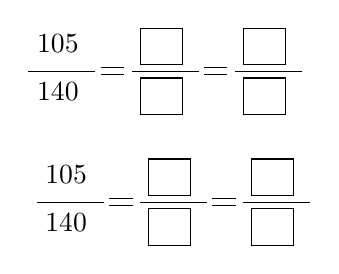
\begin{tikzpicture}[x=0.75pt,y=0.75pt,yscale=-1,xscale=1]
\draw    (31.4,70.47) -- (63.69,70.47) ;
\draw   (85.4,49.47) -- (105.69,49.47) -- (105.69,66.95) -- (85.4,66.95) -- cycle ;
\draw   (135,49.47) -- (155.29,49.47) -- (155.29,66.95) -- (135,66.95) -- cycle ;
\draw   (85.4,73.47) -- (105.69,73.47) -- (105.69,90.95) -- (85.4,90.95) -- cycle ;
\draw   (135,73.47) -- (155.29,73.47) -- (155.29,90.95) -- (135,90.95) -- cycle ;


\draw    (81.4,70.47) -- (113.69,70.47) ;

\draw    (66.4,68.47) -- (77.69,68.47) ;

\draw    (66.4,71.95) -- (77.69,71.95) ;

 
\draw    (131,70.47) -- (163.29,70.47) ;

\draw    (116,68.47) -- (127.29,68.47) ;
] 
\draw    (116,71.95) -- (127.29,71.95) ;
\draw    (35.4,133.47) -- (67.69,133.47) ;
\draw   (89.4,112.47) -- (109.69,112.47) -- (109.69,129.95) -- (89.4,129.95) -- cycle ;

\draw   (139,112.47) -- (159.29,112.47) -- (159.29,129.95) -- (139,129.95) -- cycle ;

\draw   (89.4,136.47) -- (109.69,136.47) -- (109.69,153.95) -- (89.4,153.95) -- cycle ;

\draw   (139,136.47) -- (159.29,136.47) -- (159.29,153.95) -- (139,153.95) -- cycle ;

\draw    (85.4,133.47) -- (117.69,133.47) ;

\draw    (70.4,131.47) -- (81.69,131.47) ;

\draw    (70.4,134.95) -- (81.69,134.95) ;


\draw    (135,133.47) -- (167.29,133.47) ;
 
\draw    (120,131.47) -- (131.29,131.47) ;

\draw    (120,134.95) -- (131.29,134.95) ;

\draw (34.4,51.47) node [anchor=north west][inner sep=0.75pt]   [align=left] {105};

\draw (34.4,74.47) node [anchor=north west][inner sep=0.75pt]   [align=left] {140};

\draw (38.4,137.47) node [anchor=north west][inner sep=0.75pt]   [align=left] {140};

\draw (38.4,114.47) node [anchor=north west][inner sep=0.75pt]   [align=left] {105};


\end{tikzpicture}
\end{center}
}%
\questionID {C6MDT7C}%
\question
{Find the equivalent fraction for $\frac{210}{280}$ with numerator 3.}%
\hints{
To find an equivalent fraction, we may multiply or \rule{40pt}{0.5pt} both the numerator and the denominator by the same number.\\
 To get the denominator 3, divide numerator and denominator with same number.\\\bigskip 
 
\begin{center}

\tikzset{every picture/.style={line width=0.75pt}} 
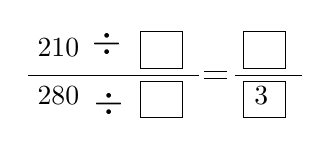
\begin{tikzpicture}[x=0.75pt,y=0.75pt,yscale=-1,xscale=1]


\draw    (41.65,36.47) -- (73.94,36.47) ;
 
\draw    (126.25,34.47) -- (137.54,34.47) ;

\draw    (126.25,37.95) -- (137.54,37.95) ;


\draw   (95.9,15.47) -- (116.19,15.47) -- (116.19,32.95) -- (95.9,32.95) -- cycle ;

\draw   (145.5,15.47) -- (165.79,15.47) -- (165.79,32.95) -- (145.5,32.95) -- cycle ;


\draw   (95.9,39.47) -- (116.19,39.47) -- (116.19,56.95) -- (95.9,56.95) -- cycle ;

\draw   (145.5,39.47) -- (165.79,39.47) -- (165.79,56.95) -- (145.5,56.95) -- cycle ;


\draw    (141.25,36.47) -- (173.54,36.47) ;

\draw    (71,36.47) -- (123.69,36.47) ;

\draw (44.9,40.47) node [anchor=north west][inner sep=0.75pt]   [align=left] {280};

\draw (44.9,17.47) node [anchor=north west][inner sep=0.75pt]   [align=left] {210};

\draw (149.33,40.67) node [anchor=north west][inner sep=0.75pt]   [align=left] {3};

\draw (71.5,13.75) node [anchor=north west][inner sep=0.75pt]  [font=\Large] [align=left] {÷};

\draw (72.25,42.5) node [anchor=north west][inner sep=0.75pt]  [font=\Large] [align=left] {÷};


\end{tikzpicture}
    
\end{center}

}%
\questionID {C6MDT12A}%
\question
{Arrange the following numbers in ascending order; 2.01, 1.2, 0.002, 0.02, 1.002\\
}%
\hints{
\begin{center}
    
\tikzset{every picture/.style={line width=0.75pt}}     

\begin{tikzpicture}[x=0.75pt,y=0.75pt,yscale=-1,xscale=1]

\draw    (164,39) -- (196.29,39) ;
 
\draw   (170,43) -- (190.29,43) -- (190.29,60.48) -- (170,60.48) -- cycle ;

\draw    (379,41) -- (411.29,41) ;

\draw   (385,45) -- (405.29,45) -- (405.29,62.48) -- (385,62.48) -- cycle ;

\draw    (555,41) -- (587.29,41) ;

\draw   (561,45) -- (581.29,45) -- (581.29,62.48) -- (561,62.48) -- cycle ;

\draw    (114,108) -- (146.29,108) ;

\draw   (120,112) -- (140.29,112) -- (140.29,129.48) -- (120,129.48) -- cycle ;

\draw    (364,113) -- (396.29,113) ;
 
\draw   (370,117) -- (390.29,117) -- (390.29,134.48) -- (370,134.48) -- cycle ;


\draw (9,16) node [anchor=north west][inner sep=0.75pt]   [align=left] {2.01 = 2 + 0.01 = 2 + };

\draw (173.67,16) node [anchor=north west][inner sep=0.75pt]   [align=left] {2};

\draw (232,91) node [anchor=north west][inner sep=0.75pt]   [align=left] {1.02 = 1 + 0.02 = };

\draw (373.67,90) node [anchor=north west][inner sep=0.75pt]   [align=left] {2};

\draw (9,86) node [anchor=north west][inner sep=0.75pt]   [align=left] {0.02 = 0.02 = \ };

\draw (123.67,85) node [anchor=north west][inner sep=0.75pt]   [align=left] {2};

\draw (467,18) node [anchor=north west][inner sep=0.75pt]   [align=left] { 0.2 = 0.2 = };

\draw (564.67,18) node [anchor=north west][inner sep=0.75pt]   [align=left] {2};

\draw (232,18) node [anchor=north west][inner sep=0.75pt]   [align=left] {1.2 = 1 + 0.2 = 1 + };

\draw (388.67,18) node [anchor=north west][inner sep=0.75pt]   [align=left] {2};

\end{tikzpicture}
\end{center}\begin{table}[H]
  \centering
\renewcommand{\arraystretch}{1.15}
    \begin{tabular}{|p{5.5cm}|p{1.5cm}|p{2.5cm}|p{3.5cm}|}
    \hline
        Expand the numbers & Ones & Tenths & Hundredths  \\
        \hline
       Least number &  &  &     \\
        \hline
        Second least number &  &  &     \\
        \hline
        Third least number &  &  &    \\
        \hline
        Fourth least number &  &  &    \\
        \hline
         Greatest number & 2 & 0 & 1   \\
        \hline
         \end{tabular}\\
\end{table}Arranging the numbers  in ascending order, we get :}%
\questionID {C6MDT12B}%
\question
{

\begin{center}
\tikzset{every picture/.style={line width=0.75pt}}      
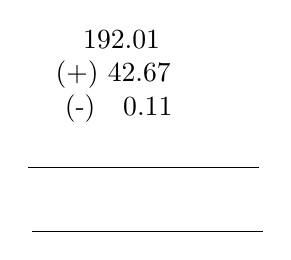
\begin{tikzpicture}[x=0.75pt,y=0.75pt,yscale=-1,xscale=1]
\draw    (266,195) -- (377,195) ;
\draw    (264,164) -- (375,164) ;
\draw (267,97) node [anchor=north west][inner sep=0.75pt]   [align=left] { \ \ \ \ \ 192.01\\ \ \ (+) 42.67\\ \ \ \ (-) \ \ 0.11};
\end{tikzpicture}
\end{center}
}%
\hints{\begin{table}[H]
  \centering
\renewcommand{\arraystretch}{1.15}
    \begin{tabular}{|p{3.5cm}|p{2.5cm}|p{1.5cm}|p{1.5cm}|p{2.5cm}|p{2.5cm}|}
    \hline
        Numbers & Hundreds & Tens & Ones & Tenths & Hundredths \\
        \hline
       192.01 &  &  &  &  & \\
        \hline
        42.67 &  &  & &  &  \\
        \hline
        Sum  &  &  &  & & \\
        \hline
         \end{tabular}\\
\end{table}

\begin{table}[H]
  \centering
\renewcommand{\arraystretch}{1.15}
    \begin{tabular}{|p{3.5cm}|p{2.5cm}|p{1.5cm}|p{1.5cm}|p{2.5cm}|p{2.5cm}|}
    \hline
        Numbers & Hundreds & Tens & Ones & Tenths & Hundredths \\
        \hline
      \rule{40pt}{0.5pt} &  &  &  & &  \\
        \hline
       0.11 &  &  & & & \\
        \hline
       Difference &  &  &  & &  \\
        \hline
         \end{tabular}\\
\end{table}}%
\questionID {C6MDT12C}%
\question
{Shop keeper had a stock of 12kg 720grams of oranges in his shop.\\
Customer 1 bought = 1kg 300grams\\
Customer 2 bought = 3kg 120grams\\
Customer 3 bought = 5kg\\
What is the remaining stock in his shop?}%
\hints{Stock of oranges in the shop : \rule{80pt}{0.5pt}\\

\begin{center}
\begin{align*}
\text{Total oranges sold} &= \text{\rule{80pt}{0.5pt} + \rule{80pt}{0.5pt} + \rule{80pt}{0.5pt} = \rule{80pt}{0.5pt}}\\
\text{Remaining stock} &= \text{Stock of oranges in the shop \rule{80pt}{0.5pt} (+/-) Total oranges sold} \\
\text{Remaining stock} &= \text{\rule{80pt}{0.5pt}}
\end{align*}
\end{center}
}%
\questionID {C6MDT13A}%
\question
{Who scored the highest mark ?\\


\bigskip{}

\tikzset{every picture/.style={line width=0.75pt}}        

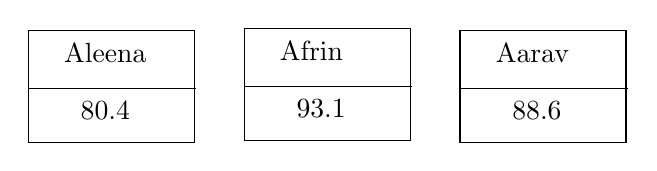
\begin{tikzpicture}[x=0.75pt,y=0.75pt,yscale=-1,xscale=1]



\draw   (212,109) -- (292,109) -- (292,163) -- (212,163) -- cycle ;
 
\draw    (212,137) -- (293,137) ;

 
\draw   (316,108) -- (396,108) -- (396,162) -- (316,162) -- cycle ;
 
\draw    (316,136) -- (397,136) ;

\draw   (420,109) -- (500,109) -- (500,163) -- (420,163) -- cycle ;

\draw    (420,137) -- (501,137) ;




\draw (228,114) node [anchor=north west][inner sep=0.75pt]   [align=left] {Aleena};
\draw (236,142) node [anchor=north west][inner sep=0.75pt]   [align=left] {80.4};
\draw (444,142) node [anchor=north west][inner sep=0.75pt]   [align=left] {88.6};
\draw (436,114) node [anchor=north west][inner sep=0.75pt]   [align=left] {Aarav};
\draw (332,113) node [anchor=north west][inner sep=0.75pt]   [align=left] {Afrin};
\draw (340,141) node [anchor=north west][inner sep=0.75pt]   [align=left] {93.1};


\end{tikzpicture}
}%
\hints{ \begin{table}[H]
  \centering
\renewcommand{\arraystretch}{1.5}
    \begin{tabular}{|p{2.5cm}|p{4.5cm}|p{1.5cm}|p{1.5cm}|p{1.5cm}|m{5cm}|}
    \hline
        \textbf{Name} & \textbf{Mark Scored}  &  \textbf{Tens} & \textbf{Ones} & \textbf{Tenths}  \\
        \hline
         & Highest mark & & &  \\
        \hline
         & Second highest mark  & & &  \\
        \hline
         & Least mark  & & &   \\
        \hline
         \end{tabular}
\end{table}
The highest mark is scored by \rule{80pt}{0.5pt}}%
\questionID {C6MDT13B}%
\question
{
Compare the following pairs of numbers using $>$ or $<$.

\bigskip{}
\tikzset{every picture/.style={line width=0.75pt}} 
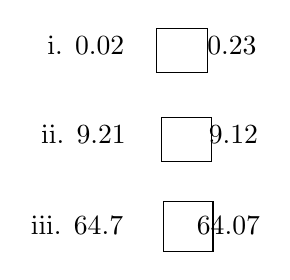
\begin{tikzpicture}[x=0.75pt,y=0.75pt,yscale=-1,xscale=1]



\draw   (273,75.6) -- (297.29,75.6) -- (297.29,97) -- (273,97) -- cycle ;

\draw   (275,118.6) -- (299.29,118.6) -- (299.29,140) -- (275,140) -- cycle ;

\draw   (276,159) -- (300,159) -- (300,183) -- (276,183) -- cycle ;



\draw (216,121) node [anchor=north west][inner sep=0.75pt]   [align=left] {ii. 9.21 \ \ \ \ \ \ \ \   9.12};

\draw (211,165) node [anchor=north west][inner sep=0.75pt]   [align=left] {iii. 64.7 \ \ \ \ \ \ \   64.07};

\draw (219,78) node [anchor=north west][inner sep=0.75pt]   [align=left] {i. 0.02 \ \ \ \ \ \ \ \  0.23};


\end{tikzpicture}}%
\hints{\begin{table}[H]
  \centering
\renewcommand{\arraystretch}{1.15}
    \begin{tabular}{|p{4.5cm}|p{1.5cm}|p{1.5cm}|p{2.5cm}|p{2.5cm}|m{5cm}|}
    \hline
        \textbf{Comparing numbers} & \textbf{Tens}  &  \textbf{Ones} & \textbf{Tenths} & \textbf{Hundredths}  \\
        \hline
         0.02 &  &   &  &   \\
        \hline
         0.23 &   &   &  &   \\
        \hline
         \end{tabular}
\end{table}
\begin{table}[H]
  \centering
\renewcommand{\arraystretch}{1.15}
    \begin{tabular}{|p{4.5cm}|p{1.5cm}|p{1.5cm}|p{2.5cm}|p{2.5cm}|m{5cm}|}
    \hline
        \textbf{Comparing numbers} & \textbf{Tens}  &  \textbf{Ones} & \textbf{Tenths} & \textbf{Hundredths}  \\
        \hline
         9.21 &  &   &  &   \\
        \hline
         9.12 &   &   &  &   \\
        \hline
         \end{tabular}
\end{table}
\begin{table}[H]
  \centering
\renewcommand{\arraystretch}{1.15}
    \begin{tabular}{|p{4.5cm}|p{1.5cm}|p{1.5cm}|p{2.5cm}|p{2.5cm}|m{5cm}|}
    \hline
        \textbf{Comparing numbers} & \textbf{Tens}  &  \textbf{Ones} & \textbf{Tenths} & \textbf{Hundredths}  \\
        \hline
         64.7 &  &   &  &   \\
        \hline
         64.07 &   &   &  &   \\
        \hline
         \end{tabular}
\end{table}}%
\questionID {C6MDT13C}%
\question
{Pick the numbers which are above 8521.02. \bigskip{} \tikzset{every picture/.style={line width=0.75pt}} 

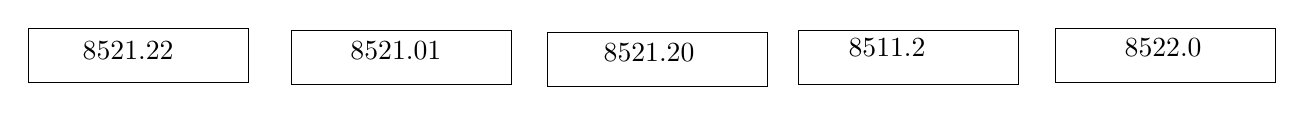
\begin{tikzpicture}[x=0.75pt,y=0.75pt,yscale=-1,xscale=1]



\draw   (21,30) -- (127,30) -- (127,56) -- (21,56) -- cycle ;

\draw   (148,31) -- (254,31) -- (254,57) -- (148,57) -- cycle ;

\draw   (271,32) -- (377,32) -- (377,58) -- (271,58) -- cycle ;

\draw   (392,31) -- (498,31) -- (498,57) -- (392,57) -- cycle ;

\draw   (516,30) -- (622,30) -- (622,56) -- (516,56) -- cycle ;



\draw (46,35) node [anchor=north west][inner sep=0.75pt]   [align=left] {8521.22};

\draw (175,35) node [anchor=north west][inner sep=0.75pt]   [align=left] {8521.01};

\draw (297,36) node [anchor=north west][inner sep=0.75pt]   [align=left] {8521.20};

\draw (415,34) node [anchor=north west][inner sep=0.75pt]   [align=left] {8511.2};

\draw (548,34) node [anchor=north west][inner sep=0.75pt]   [align=left] {8522.0};


\end{tikzpicture}}%
\hints{\begin{table}[H]
  \centering
\renewcommand{\arraystretch}{1.15}
    \begin{tabular}{|p{3.5cm}|p{2.5cm}|p{2cm}|p{2cm}|p{1.5cm}|p{1.5cm}|p{2.5cm}|p{4cm}|m{4cm}|}
    \hline
        \textbf{Expand numbers} & \textbf{Thousands}  &  \textbf{Hundreds} & \textbf{Tens} & \textbf{Ones} & \textbf{Tenths} & \textbf{Hundredths} \\
        \hline
         8521.22 &  &   &  &  & &  \\
        \hline
        8521.01 &   &   &  &  & & \\
        \hline
         8521.20 &  &   &  &  &  & \\
        \hline
        8511.2 &   &   &  &  & &  \\
        \hline
        8522.0  &  &   &  &  & &   \\
        \hline
         \end{tabular}
\end{table}}%
\qrdes {Hi, here in this video we going to learn how to divide a number and divisibility rule.}%
\qr {C6MDT3.png}%
\questionID {C6MDT3A}%
\question
{Pick the common multiple of 4 and 8. 

\begin{center}
\tikzset{every picture/.style={line width=0.75pt}}
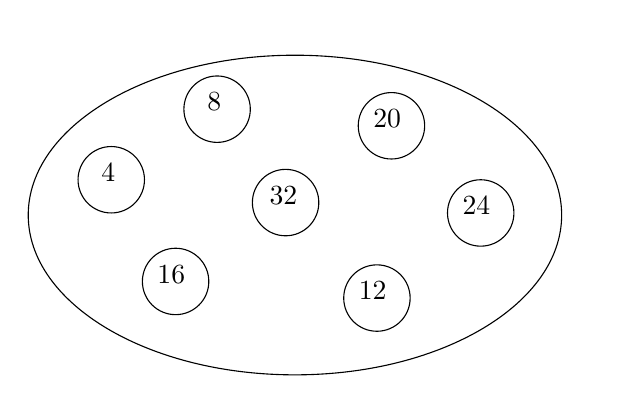
\begin{tikzpicture}[x=0.75pt,y=0.75pt,yscale=-1,xscale=1]
\draw   (124,164) .. controls (124,155.16) and (131.16,148) .. (140,148) .. controls (148.84,148) and (156,155.16) .. (156,164) .. controls (156,172.84) and (148.84,180) .. (140,180) .. controls (131.16,180) and (124,172.84) .. (124,164) -- cycle ;
\draw   (100,181) .. controls (100,138.47) and (157.53,104) .. (228.5,104) .. controls (299.47,104) and (357,138.47) .. (357,181) .. controls (357,223.53) and (299.47,258) .. (228.5,258) .. controls (157.53,258) and (100,223.53) .. (100,181) -- cycle ;
\draw   (155,213) .. controls (155,204.16) and (162.16,197) .. (171,197) .. controls (179.84,197) and (187,204.16) .. (187,213) .. controls (187,221.84) and (179.84,229) .. (171,229) .. controls (162.16,229) and (155,221.84) .. (155,213) -- cycle ;
\draw   (175,130) .. controls (175,121.16) and (182.16,114) .. (191,114) .. controls (199.84,114) and (207,121.16) .. (207,130) .. controls (207,138.84) and (199.84,146) .. (191,146) .. controls (182.16,146) and (175,138.84) .. (175,130) -- cycle ;
\draw   (208,175) .. controls (208,166.16) and (215.16,159) .. (224,159) .. controls (232.84,159) and (240,166.16) .. (240,175) .. controls (240,183.84) and (232.84,191) .. (224,191) .. controls (215.16,191) and (208,183.84) .. (208,175) -- cycle ;
\draw   (259,138) .. controls (259,129.16) and (266.16,122) .. (275,122) .. controls (283.84,122) and (291,129.16) .. (291,138) .. controls (291,146.84) and (283.84,154) .. (275,154) .. controls (266.16,154) and (259,146.84) .. (259,138) -- cycle ;
\draw   (302,180) .. controls (302,171.16) and (309.16,164) .. (318,164) .. controls (326.84,164) and (334,171.16) .. (334,180) .. controls (334,188.84) and (326.84,196) .. (318,196) .. controls (309.16,196) and (302,188.84) .. (302,180) -- cycle ;
\draw   (252,221) .. controls (252,212.16) and (259.16,205) .. (268,205) .. controls (276.84,205) and (284,212.16) .. (284,221) .. controls (284,229.84) and (276.84,237) .. (268,237) .. controls (259.16,237) and (252,229.84) .. (252,221) -- cycle ;
\draw (134,155) node [anchor=north west][inner sep=0.75pt]   [align=left] {4};
\draw (373,91) node [anchor=north west][inner sep=0.75pt]   [align=left] {};
\draw (185,121) node [anchor=north west][inner sep=0.75pt]   [align=left] {8};
\draw (161,204) node [anchor=north west][inner sep=0.75pt]   [align=left] {16};
\draw (215,166) node [anchor=north west][inner sep=0.75pt]   [align=left] {32};
\draw (265,129) node [anchor=north west][inner sep=0.75pt]   [align=left] {20};
\draw (308,171) node [anchor=north west][inner sep=0.75pt]   [align=left] {24};
\draw (258,212) node [anchor=north west][inner sep=0.75pt]   [align=left] {12};
\end{tikzpicture}
    
\end{center}
}%
\hints{The multiples of 4 are \rule{20pt}{0.5pt}, \rule{20pt}{0.5pt}, \rule{20pt}{0.5pt}, \rule{20pt}{0.5pt}, \rule{20pt}{0.5pt}, \rule{20pt}{0.5pt}, \rule{20pt}{0.5pt}, \rule{20pt}{0.5pt} \\
The multiples of 8 are \rule{20pt}{0.5pt}, \rule{20pt}{0.5pt}, \rule{20pt}{0.5pt}, \rule{20pt}{0.5pt}, \rule{20pt}{0.5pt}, \rule{20pt}{0.5pt}, \rule{20pt}{0.5pt}, \rule{20pt}{0.5pt} \\
The common multiples of 4 and 8 in the above circle are \rule{20pt}{0.5pt}, \rule{20pt}{0.5pt}, \rule{20pt}{0.5pt} and \rule{20pt}{0.5pt}.}
%
\questionID {C6MDT3B}%
\question
{Find the LCM of 50, twice of 50 and thrice of 50.}%
\hints{Twice of 50  = 2 x \rule{20pt}{0.5pt}  = \rule{40pt}{0.5pt}\\
Thrice of 50 = 3 x \rule{20pt}{0.5pt} = \rule{40pt}{0.5pt}\\
Complete the division using least common multiple.\\
{\begin{center}
\tikzset{every picture/.style={line width=0.75pt}}      

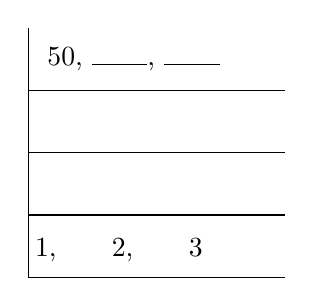
\begin{tikzpicture}[x=0.75pt,y=0.75pt,yscale=-1,xscale=1]
\draw    (157,238) -- (157,268) ;
\draw    (157,238) -- (280.8,238) ;
\draw    (157,268) -- (280.8,268) ;
\draw    (157,208) -- (157,238) ;
\draw    (157,208) -- (280.8,208) ;
\draw    (157,178) -- (157,192) -- (157,208) ;
\draw    (157,178) -- (280.8,178) ;
\draw    (157,148) -- (157,178) ;
\draw (165,156) node [anchor=north west][inner sep=0.75pt]   [align=left] {50, \rule{20pt}{0.5pt}, \rule{20pt}{0.5pt}};
\draw (165,156) node [anchor=north west][inner sep=0.75pt]   [align=left] {};
\draw (159,213) node [anchor=north west][inner sep=0.75pt]   [align=left] {};
\draw (159,248) node [anchor=north west][inner sep=0.75pt]   [align=left] { 1,\qquad  2,\qquad 3};
\end{tikzpicture}
\end{center}}
The LCM of 50, twice of 50 and thrice of 50 is 2 $\times$ 3 $\times$ \rule{40pt}{0.5pt} $\times$ \rule{40pt}{0.5pt}\\}%
\questionID {C6MDT3C}%
\question
{Find the least number which when divided by 20, 40 and 60 leaves a remainder 3 in each case. }%
\hints{Complete the division using least common multiple.\\
\begin{center}
\tikzset{every picture/.style={line width=0.75pt}}        
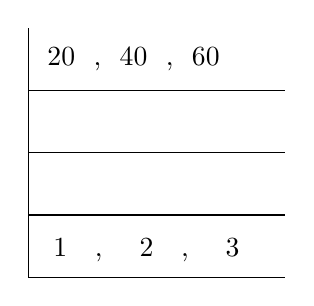
\begin{tikzpicture}[x=0.75pt,y=0.75pt,yscale=-1,xscale=1]
\draw    (161,164) -- (161,194) ;
\draw    (161,164) -- (284.8,164) ;
\draw    (161,194) -- (284.8,194) ;
\draw    (161,134) -- (161,164) ;
\draw    (161,134) -- (284.8,134) ;
\draw    (161,104) -- (161,118) -- (161,134) ;
\draw    (161,104) -- (284.8,104) ;
\draw    (161,74) -- (161,104) ;
\draw (169,82) node [anchor=north west][inner sep=0.75pt]   [align=left] {20 \ , \ 40 \ , \ 60};
\draw (165,112) node [anchor=north west][inner sep=0.75pt]   [align=left] {};
\draw (163,139) node [anchor=north west][inner sep=0.75pt]   [align=left] {};
\draw (163,174) node [anchor=north west][inner sep=0.75pt]   [align=left] { \ \ 1 \ \ , \ \ \ 2 \ \ , \ \ \ 3 \ \ };
\end{tikzpicture}\\
\end{center}
The LCM of 20, 40 and 60 is \rule{80pt}{0.5pt}.\\
To find the least number which when divided by 20, 40 and 60 leaves a remainder 3 in each case then,\\
(The LCM of 20, 40 and 60) \rule{40pt}{0.5pt} + \rule{40pt}{0.5pt} = \rule{40pt}{0.5pt} \\

}%
\qrdes {Hi, here in this video we going to learn what is angle, different types of angles and how to calculate the angles.}%
\qr {C6MDT4.png}%
\questionID {C6MDT4A}%
\question
{Tick the correct answer.\\25 is a (Prime number/Composite number)}%
\hints{To check whether it is a prime or a composite number.
\begin{center}
{\begin{tabular}{|c|}

    \hline
       \rule{20pt}{0.5pt} x 1 = 25 \\
    \hline
   \rule{20pt}{0.5pt} x \rule{20pt}{0.5pt}  = 25 \\
    \hline
   \rule{20pt}{0.5pt} x \rule{20pt}{0.5pt}  = 25\\
    \hline
    \end{tabular}}
\end{center}
The number 25 has \rule{40pt}{0.5pt} factors.\\
The factors of 25 are \rule{40pt}{0.5pt}.\\
The number 25 is a \rule{40pt}{0.5pt} number.

}%
\questionID {C6MDT4B}%
\question
{From the given numbers, write down the prime numbers and composite numbers separately.
\begin{center}

\tikzset{every picture/.style={line width=0.75pt}}         
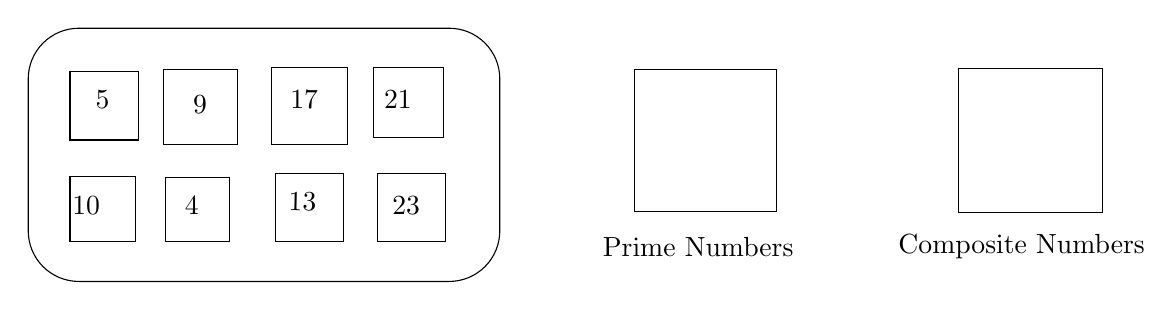
\begin{tikzpicture}[x=0.75pt,y=0.75pt,yscale=-1,xscale=1]
\draw   (47,85.8) .. controls (47,72.32) and (57.92,61.4) .. (71.4,61.4) -- (249.8,61.4) .. controls (263.28,61.4) and (274.2,72.32) .. (274.2,85.8) -- (274.2,159) .. controls (274.2,172.48) and (263.28,183.4) .. (249.8,183.4) -- (71.4,183.4) .. controls (57.92,183.4) and (47,172.48) .. (47,159) -- cycle ;
\draw   (67.15,82.4) -- (100,82.4) -- (100,115.25) -- (67.15,115.25) -- cycle ;
\draw   (215.15,131.4) -- (248,131.4) -- (248,164.25) -- (215.15,164.25) -- cycle ;
\draw   (112.15,81.4) -- (148,81.4) -- (148,117.25) -- (112.15,117.25) -- cycle ;
\draw   (213.15,80.4) -- (247,80.4) -- (247,114.25) -- (213.15,114.25) -- cycle ;
\draw   (67.15,132.8) -- (98.6,132.8) -- (98.6,164.25) -- (67.15,164.25) -- cycle ;
\draw   (166.15,131.4) -- (199,131.4) -- (199,164.25) -- (166.15,164.25) -- cycle ;
\draw   (113.15,133.4) -- (144,133.4) -- (144,164.25) -- (113.15,164.25) -- cycle ;
\draw   (164.15,80.4) -- (201,80.4) -- (201,117.25) -- (164.15,117.25) -- cycle ;
\draw   (339,81.4) -- (407.4,81.4) -- (407.4,149.8) -- (339,149.8) -- cycle ;
\draw   (495,80.8) -- (564.4,80.8) -- (564.4,150.2) -- (495,150.2) -- cycle ;
\draw (78.15,90.4) node [anchor=north west][inner sep=0.75pt]   [align=left] {5};
\draw (125.15,92.4) node [anchor=north west][inner sep=0.75pt]   [align=left] {9};
\draw (217.15,90.4) node [anchor=north west][inner sep=0.75pt]   [align=left] { 21};
\draw (67,141.4) node [anchor=north west][inner sep=0.75pt]   [align=left] { 10};
\draw (121.15,141.4) node [anchor=north west][inner sep=0.75pt]   [align=left] { 4};
\draw (171.34,139.19) node [anchor=north west][inner sep=0.75pt]  [rotate=-1.27] [align=left] {13};
\draw (221.15,141.4) node [anchor=north west][inner sep=0.75pt]   [align=left] {23};
\draw (172,90.4) node [anchor=north west][inner sep=0.75pt]   [align=left] {17};
\draw (322.6,160.8) node [anchor=north west][inner sep=0.75pt]   [align=left] {Prime Numbers};
\draw (465,159.6) node [anchor=north west][inner sep=0.75pt]   [align=left] {Composite Numbers};
\end{tikzpicture}

\end{center}
}%
\hints{
Prime numbers are numbers which has  \rule{80pt}{0.5pt} factors.\\
Composite numbers are numbers which has  \rule{80pt}{0.5pt} factors.
\\
\begin{align*}
  \text {Factors of 5} &: \text {1 and 5  -  2 factors}  
\\ \text {Factors of 9} &: \rule{80pt}{0.5pt} 
\\ \text {Factors of 17} &: \rule{80pt}{0.5pt} 
\\ \text {Factors of 21} &: \rule{80pt}{0.5pt} 
\\ \text {Factors of 10} &: \rule{80pt}{0.5pt}  
\\ \text {Factors of 4} &: \rule{80pt}{0.5pt}  
\\ \text {Factors of 13} &: \rule{80pt}{0.5pt}  
\\ \text {Factors of 23} &: \rule{80pt}{0.5pt}   
\end{align*}
}%
\questionID {C6MDT4C}%
\question
{31 is the sum of three consecutive prime numbers. What are the three prime numbers?}%
\hints{(The LCM of 20, 40 and 60) \rule{40pt}{0.5pt} + \rule{40pt}{0.5pt} = \rule{40pt}{0.5pt} \\ 
Adding first 3 prime numbers (2, 3, 5) : 2 + 3 + 5 = \rule{40pt}{0.5pt}\\
Adding next 3 prime numbers (3, 5, 7) : \rule{80pt}{0.5pt}\\ 
Adding next 3 prime numbers  : \rule{80pt}{0.5pt} \\ 
Adding next 3 prime numbers  : \rule{80pt}{0.5pt} \\ 
31 is the sum of three consecutive prime numbers, they are \rule{40pt}{0.5pt}, \rule{40pt}{0.5pt} and \rule{40pt}{0.5pt}.
}%
\end{document}